\chapter{Experiments \& Evaluation}
An important test for any filter\todoCitation{} \todoResearch{convolutions in furior space, think Jaehne}, is to apply the filter iteratively upon a Dirac delta function\todoCitation{}.
\section{Synthetic Data}
Synthetic Examples are generated with ideal vertices, unlike acquired examples.

\subsection{Random Noise Function}\todoResearch{Currently, no meshes exist for research}

\subsection{Vector Fields}\todoResearch{Set up: choose color with different RGB, like Cyan. Add noise to each channel. Use filter to process each channel seperately and display results.}

\subsection{A Flat surface with Dirac Delta function}
\subsubsection{Square Tesselation, two triangles}
\begin{figure}[ht]
\ffigbox
	{\begin{subfigure}[b]{0.48\linewidth}
		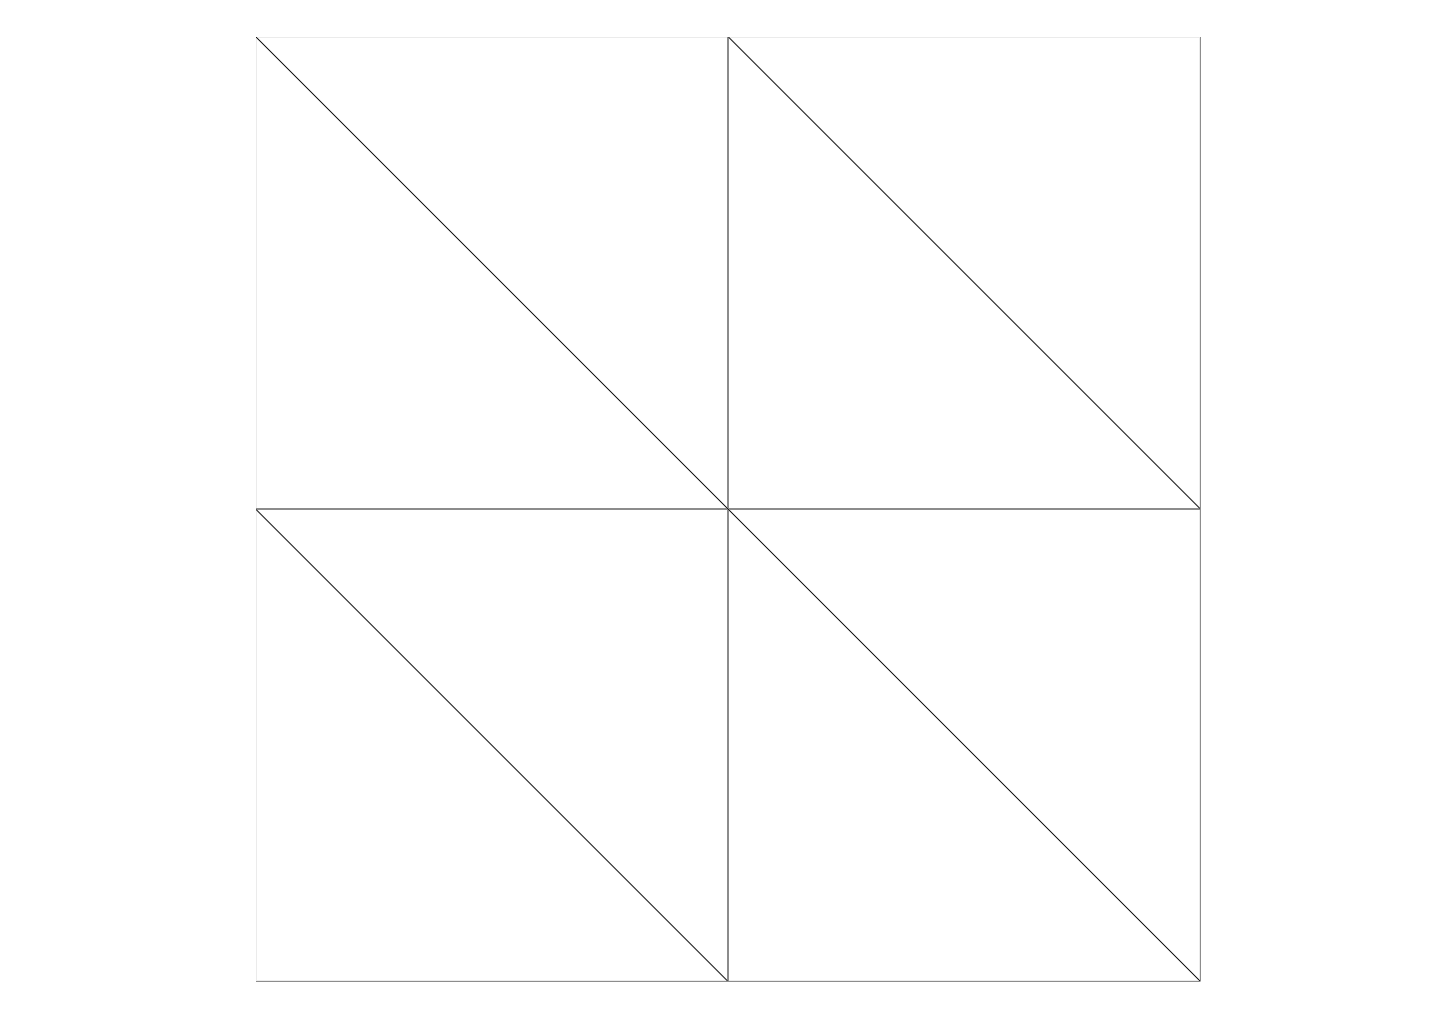
\includegraphics[width=1.0\linewidth,height=0.32\textheight,keepaspectratio]{data/synthetic_meshes/square_tesselation_2tri_Dirac_delta_1_v9_f8_wireframe.png}
		\caption{Sq2 v9\_f8 wireframe}\label{fig:sq2.a}
	\end{subfigure}
	\begin{subfigure}[b]{0.48\linewidth}
		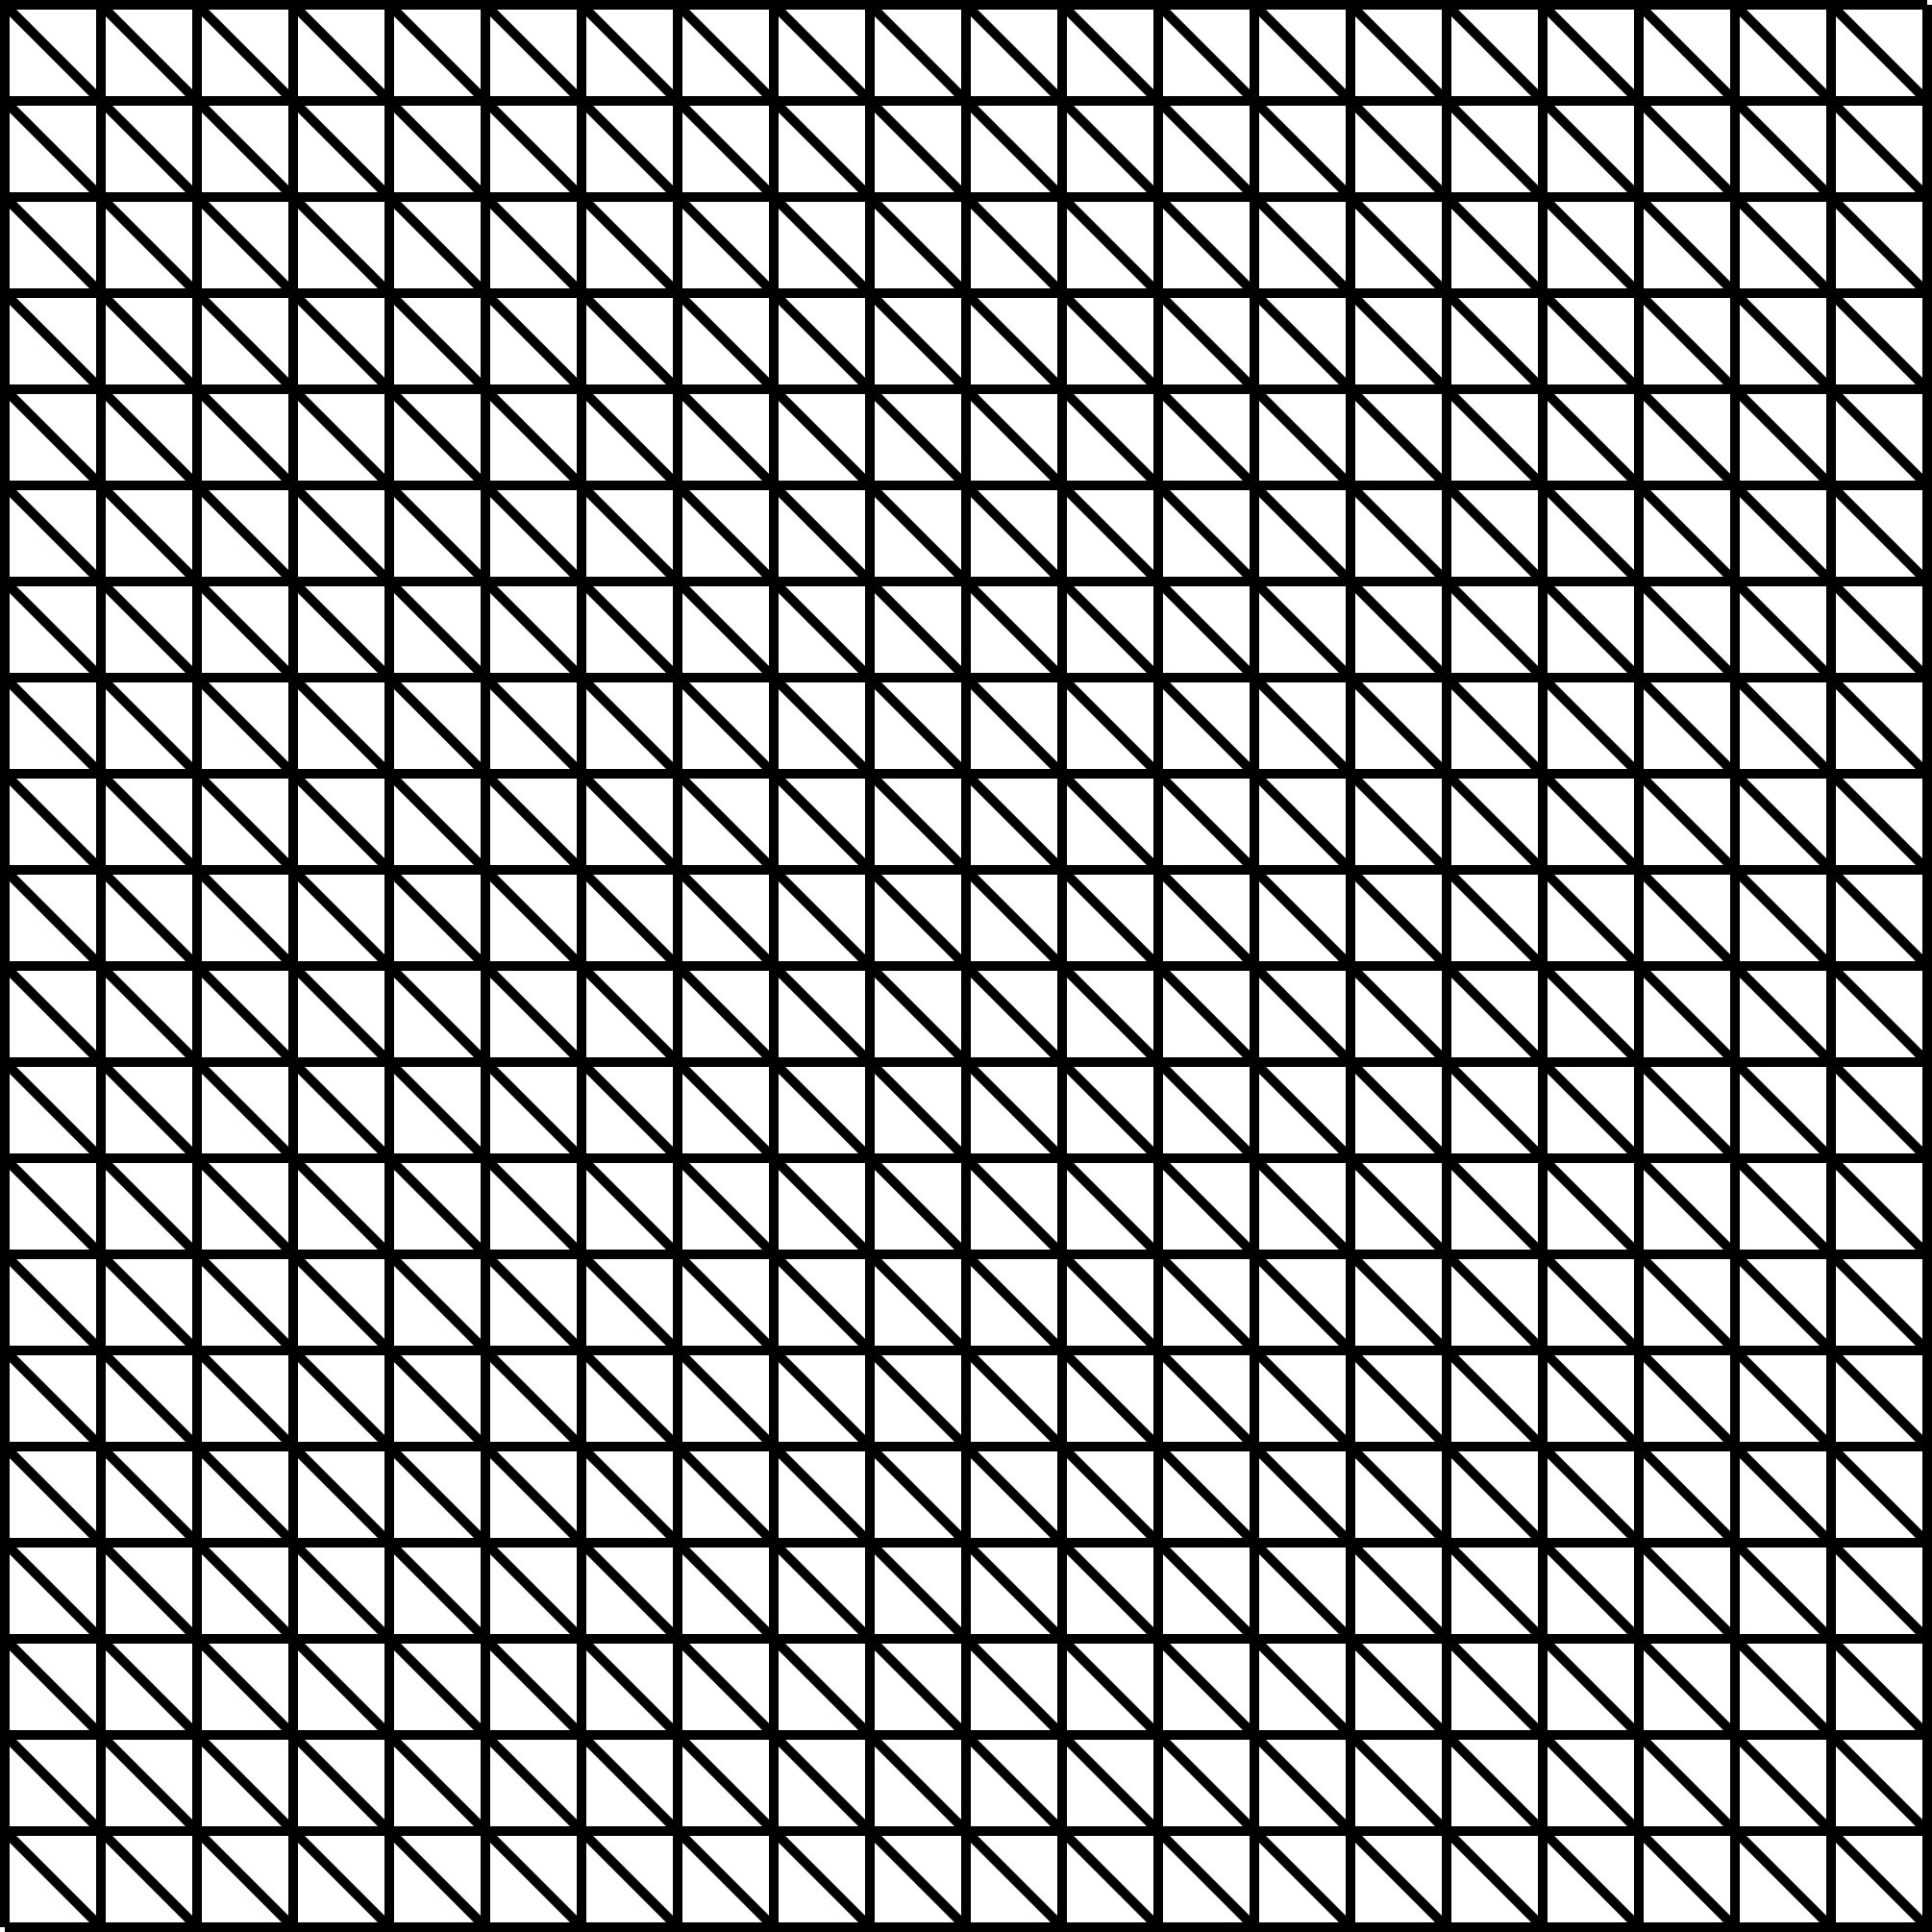
\includegraphics[width=1.0\linewidth,height=0.32\textheight,keepaspectratio]{data/synthetic_meshes/square_tesselation_2tri_Dirac_delta_10_v441_f800_wireframe.png}
		\caption{Sq2 v441\_f800 wireframe}\label{fig:sq2.b}
	\end{subfigure}

	\bigskip
	\begin{subfigure}[b]{0.48\linewidth}
		
\includegraphics[width=1.0\linewidth,height=0.32\textheight,keepaspectratio]{data/synthetic_meshes/square_tesselation_2tri_Dirac_delta_1_v9_f8_funcvals_0iter_crop.png}
		\caption{Sq2 v9\_f8 iter 0}\label{fig:sq2.c}
	\end{subfigure}
	\begin{subfigure}[b]{0.48\linewidth}
		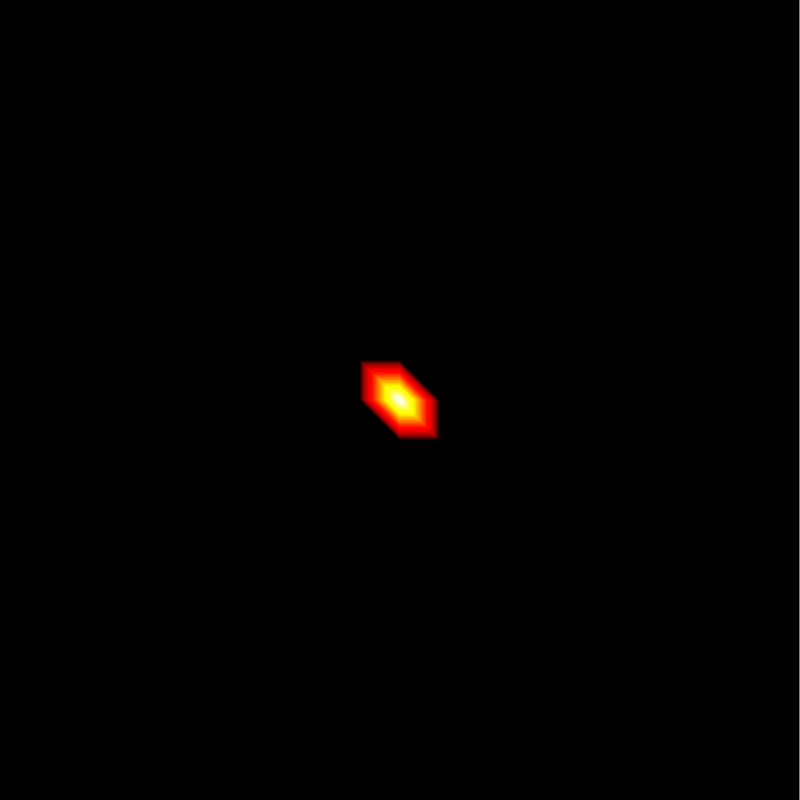
\includegraphics[width=1.0\linewidth,height=0.32\textheight,keepaspectratio]{data/synthetic_meshes/square_tessellation_2tri_Dirac_delta_10_v441_f800_funcvals_0iter.png}
		\caption{Sq2 v441\_f800 iter 0}\label{fig:sq2.d}
	\end{subfigure}

	\bigskip
	\begin{subfigure}[b]{0.48\linewidth}
		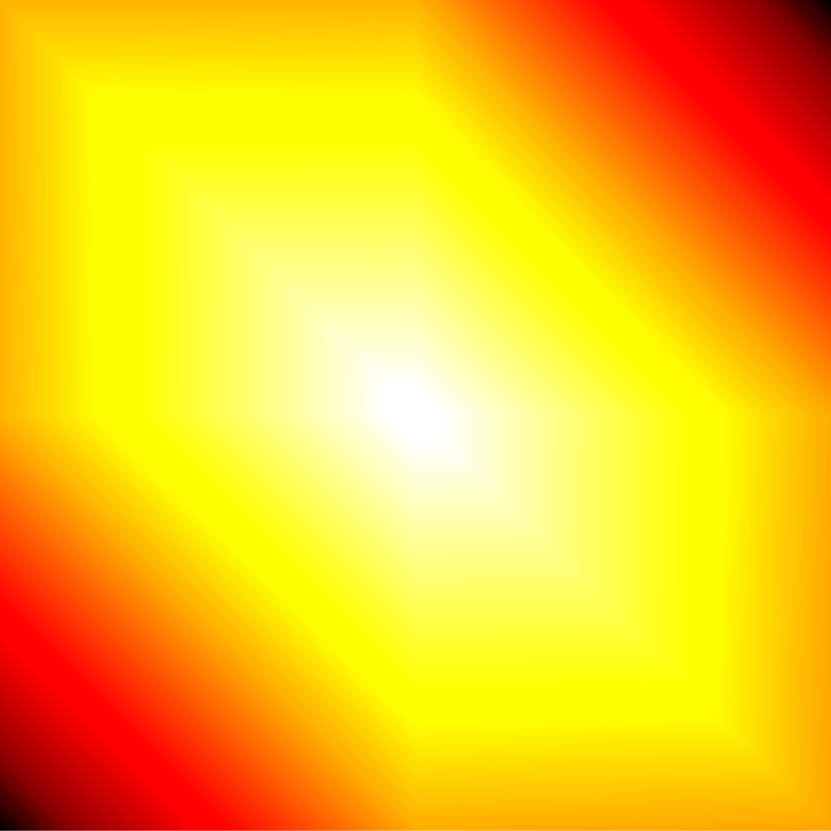
\includegraphics[width=1.0\linewidth,height=0.32\textheight,keepaspectratio]{data/synthetic_meshes/square_tesselation_2tri_Dirac_delta_1_v9_f8_funcvals_1iter_crop.png}
		\caption{Sq2 v9\_f8 iter 1}\label{fig:sq2.e}
	\end{subfigure}
	\begin{subfigure}[b]{0.48\linewidth}
		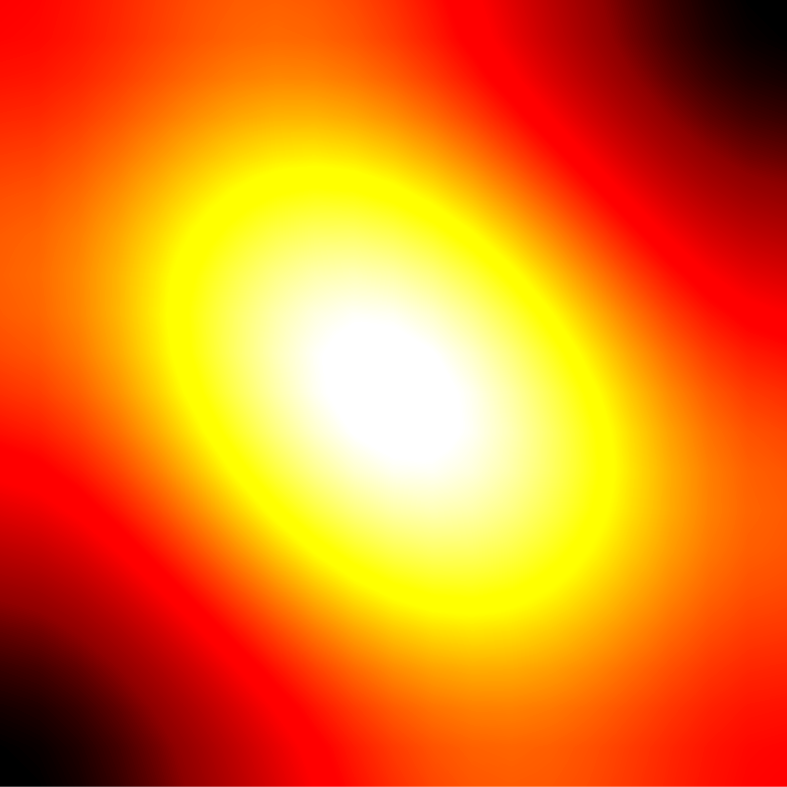
\includegraphics[width=1.0\linewidth,height=0.32\textheight,keepaspectratio]{data/synthetic_meshes/square_tessellation_2tri_Dirac_delta_10_v441_f800_funcvals_100iter.png}
		\caption{Sq2 v441\_f800 iter 100}\label{fig:sq2.f}
	\end{subfigure}}
	{\caption[Synthetic Square, 2 triangles, Dirac delta function]{A synthetic square, subdivided by triangles, with a Dirac delta function applied: (a) wireframe (b) colored by function value before filter (c) colored by function value after 1000 iterations
%GigaMesh~\cite{Mara10} with function values colored with the Improved Hot colorramp, exported as png after disabling the background grid [f7], maximizing the window, disabling screenshot cropping, as well as rejecting tiled rendering, finally cropping to content in GIMP.
	}\label{fig:sq2}}
\end{figure}
\todoCitation{}
\todoResearch{Why does sq2 10 need 100 iters to match sq 1 at 1 iters?}
\todoStyle{Why does sq2 1 iters 0 get differnt spacing?}
\todoStyle{Adjusting height, shrinks width => images no longer centered in their columns}

\subsubsection{Square grid, four triangles}

\subsubsection{Hexagonal grid}
\begin{figure}[ht]
\ffigbox
	{\begin{subfigure}[b]{0.48\linewidth}
		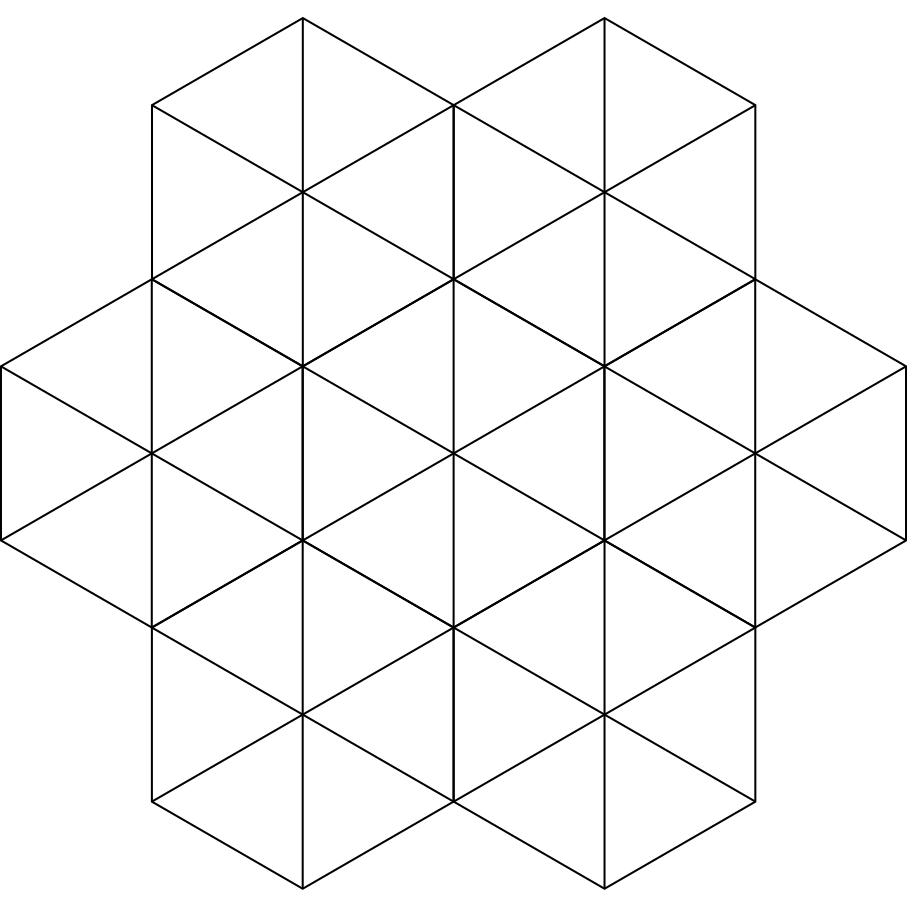
\includegraphics[width=1.0\linewidth,height=0.3\textheight,keepaspectratio]{data/synthetic_meshes/hexagonal_tessellation_Dirac_delta_1_v31_f42_wireframe.png}
		\caption{Hex v31\_f42 wireframe}\label{fig:hex.a}
	\end{subfigure}
	\begin{subfigure}[b]{0.48\linewidth}
		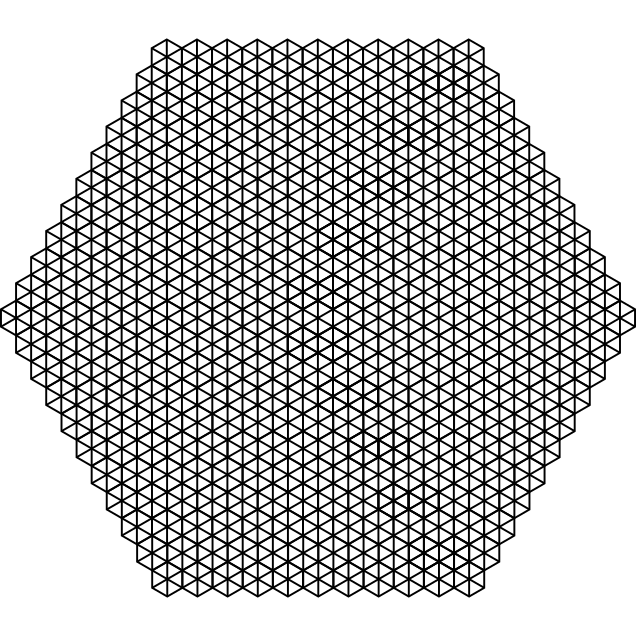
\includegraphics[width=1.0\linewidth,height=0.3\textheight,keepaspectratio]{data/synthetic_meshes/hexagonal_tessellation_Dirac_delta_10_v1057_f1986_wireframe.png}
		\caption{Hex v1057\_f1986 wireframe}\label{fig:hex.b}
	\end{subfigure}

	\bigskip
	\begin{subfigure}[b]{0.48\linewidth}
		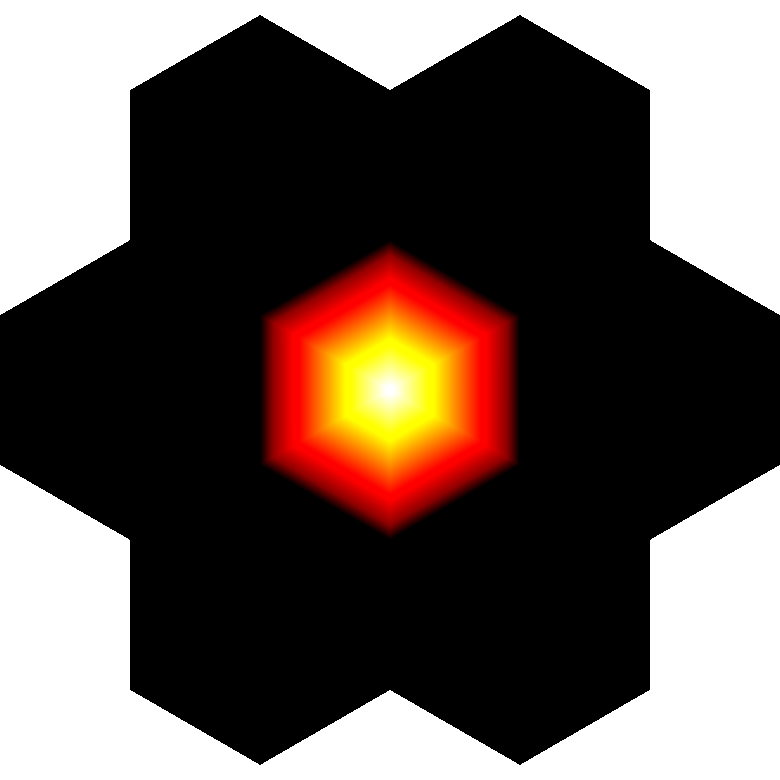
\includegraphics[width=1.0\linewidth,height=0.3\textheight,keepaspectratio]{data/synthetic_meshes/hexagonal_tessellation_Dirac_delta_1_v31_f42_funcvals_0iter_crop.png}
		\caption{Hex v31\_f42 iter 0}\label{fig:hex.c}
	\end{subfigure}
	\begin{subfigure}[b]{0.48\linewidth}
		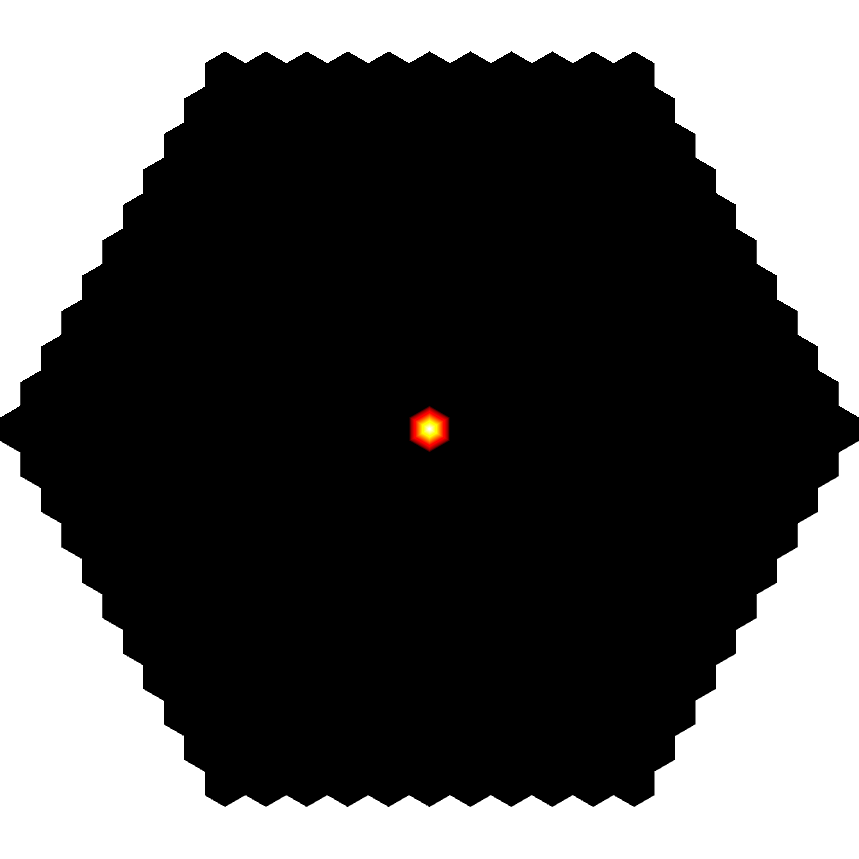
\includegraphics[width=1.0\linewidth,height=0.3\textheight,keepaspectratio]{data/synthetic_meshes/hexagonal_tessellation_Dirac_delta_10_v1057_f1986_funcvals_0iter_crop.png}
		\caption{Hex v1057\_f1986 iter 0}\label{fig:hex.d}
	\end{subfigure}

	\bigskip
	\begin{subfigure}[b]{0.48\linewidth}
		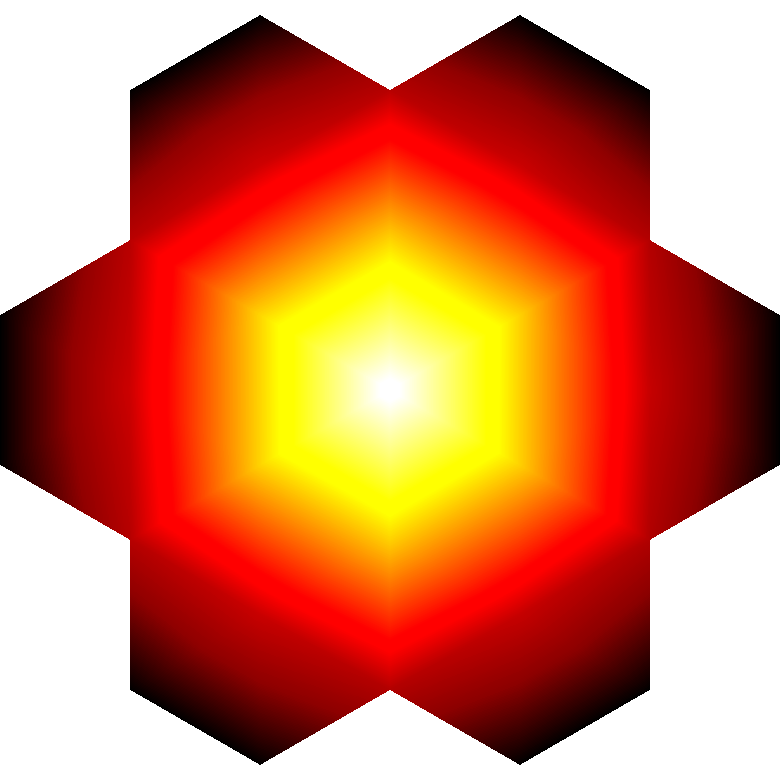
\includegraphics[width=1.0\linewidth,height=0.3\textheight,keepaspectratio]{data/synthetic_meshes/hexagonal_tessellation_Dirac_delta_1_v31_f42_funcvals_2iter_crop.png}
		\caption{Hex v31\_f42 iter 2}\label{fig:hex.e}
	\end{subfigure}
	\begin{subfigure}[b]{0.48\linewidth}
		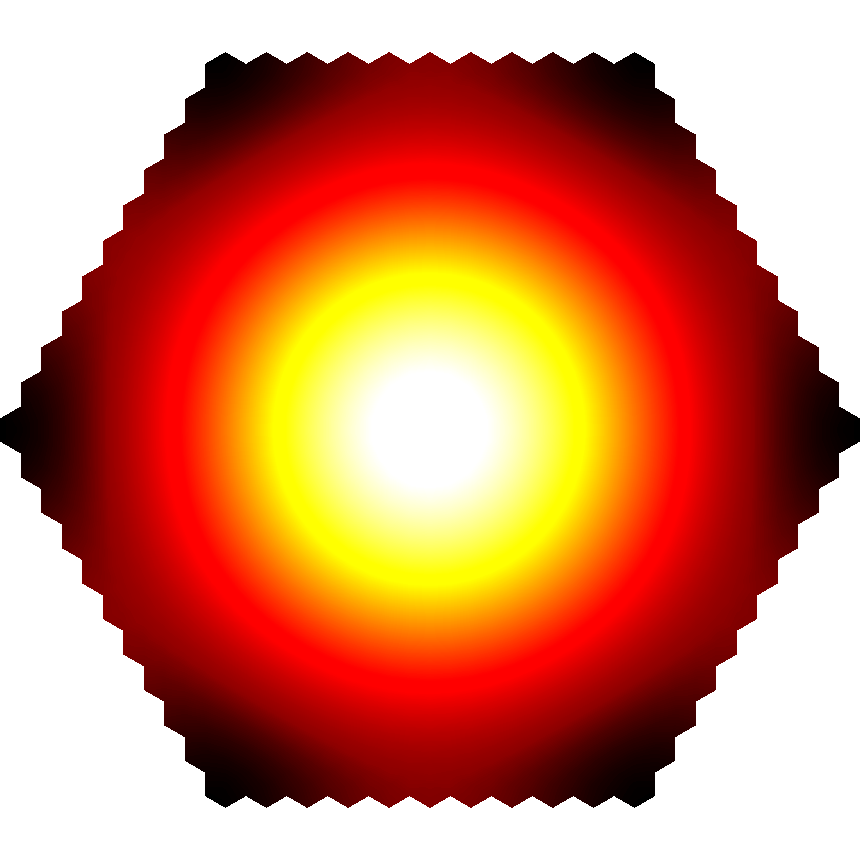
\includegraphics[width=1.0\linewidth,height=0.3\textheight,keepaspectratio]{data/synthetic_meshes/hexagonal_tessellation_Dirac_delta_10_v1057_f1986_funcvals_200iter_crop.png}
		\caption{Hex v1057\_f1986 iter 200}\label{fig:hex.f}
	\end{subfigure}}
	{\caption[Synthetic Hexagonal Tessellations, Dirac delta function]{A synthetic hexagonal tessellation, subdivided by triangles, with a Dirac delta function applied: (a) v31 f42 wireframe (b) v1057 f1986 wireframe (c) v31 f42 colored by function value before filter (d) v1057 f1986 colored by function value before filter (e) v31 f42 colored by function value after 2 iterations (e) v1057 f1986 colored by function value after 200 iterations.
% All using the colorramp "Hot (improved)"~\cite[p.~???]{Brewer2003}~\cite[p.~19]{Giga17}, visualized using GigaMesh~\cite{Mara10}, exported as png after disabling the background grid [f7], maximizing the window, disabling screenshot cropping, as well as rejecting tiled rendering, finally cropping to content in GIMP.
	}\label{fig:hex}}
\end{figure}
\todoCitation{}

\subsubsection{Random vertices within a circle}
\begin{figure}[ht]
\ffigbox
	{\begin{subfigure}[b]{0.48\linewidth}
		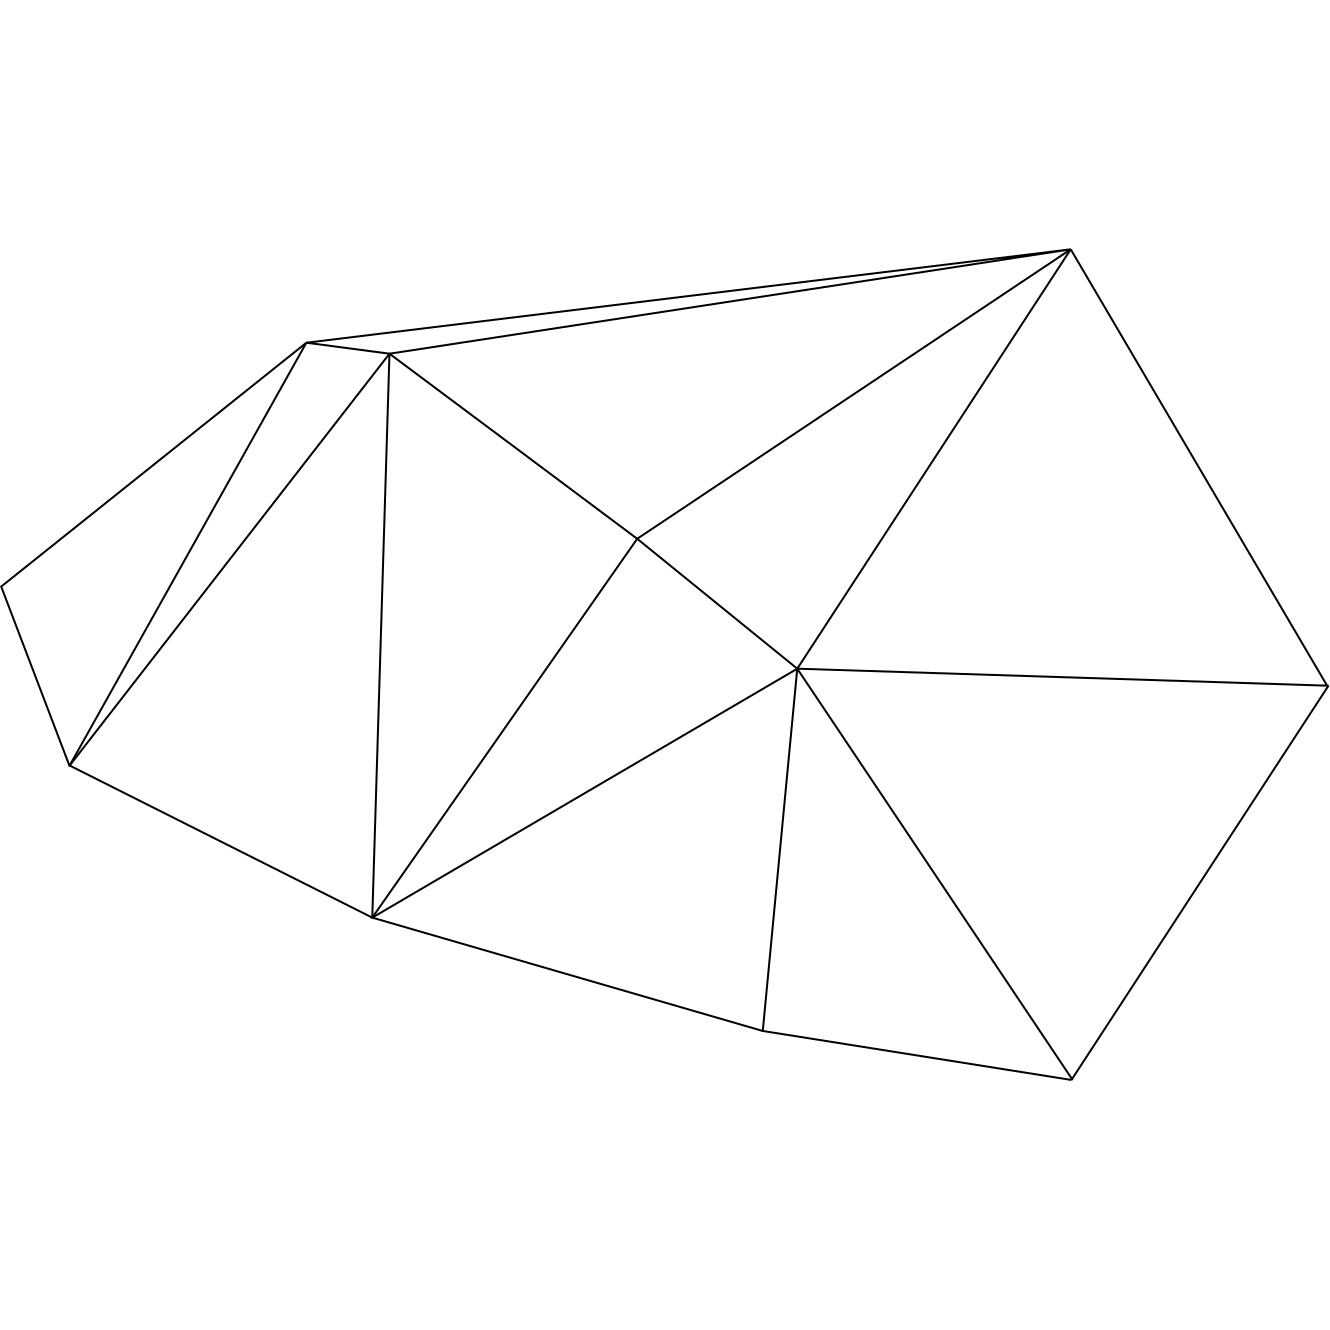
\includegraphics[width=1.0\linewidth,height=0.3\textheight,keepaspectratio]{data/synthetic_meshes/random_circle_tessellation_Dirac_delta_1_v11_f12_wireframe.png}
		\caption{R.Circ v11\_f12 wireframe}\label{fig:rcirc.a}
	\end{subfigure}
	\begin{subfigure}[b]{0.48\linewidth}
		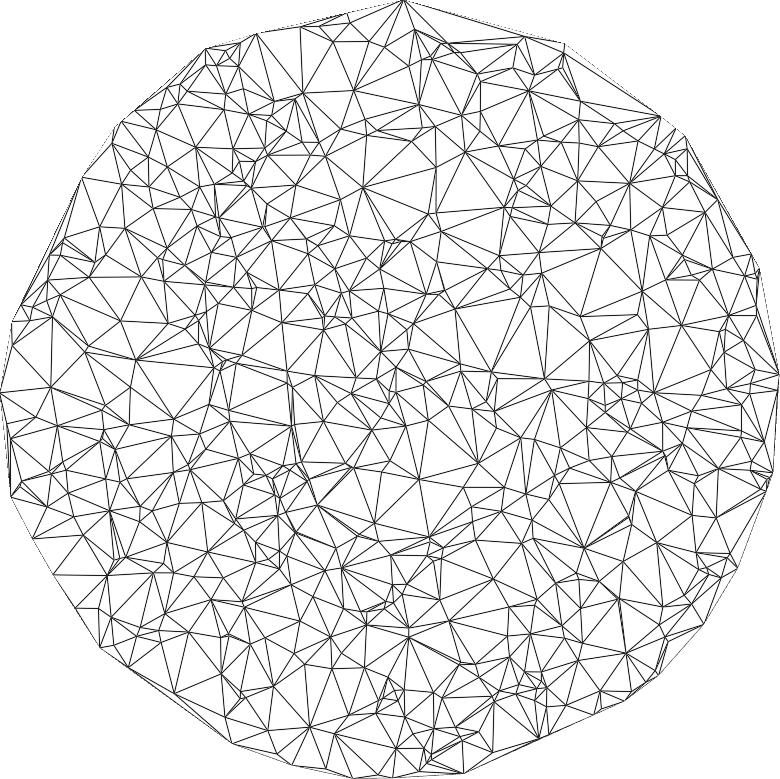
\includegraphics[width=1.0\linewidth,height=0.3\textheight,keepaspectratio]{data/synthetic_meshes/random_circle_tessellation_Dirac_delta_10_v641_f1252_wireframe.png}
		\caption{R.Circ v641\_f1252 wireframe}\label{fig:rcirc.b}
	\end{subfigure}

	\bigskip
	\begin{subfigure}[b]{0.48\linewidth}
		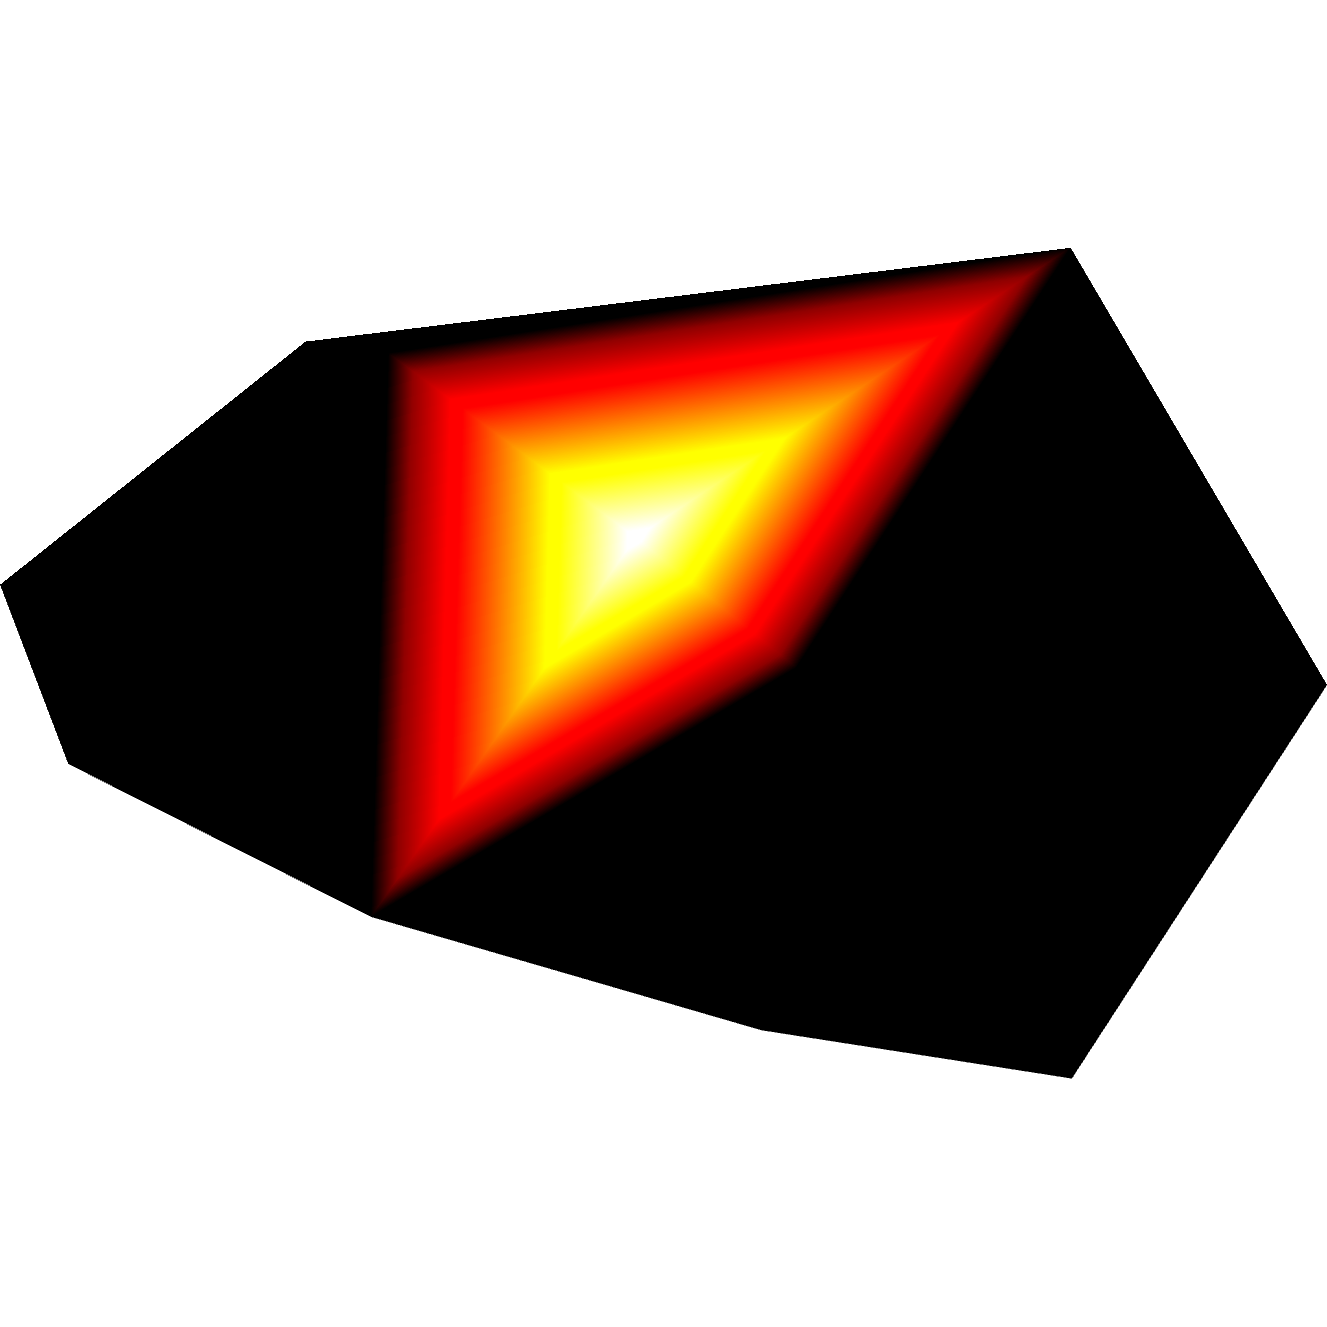
\includegraphics[width=1.0\linewidth,height=0.3\textheight,keepaspectratio]{data/synthetic_meshes/random_circle_tessellation_Dirac_delta_1_v11_f12_funcvals_0iter.png}
		\caption{R.Circ v11\_f12 iter 0}\label{fig:rcirc.c}
	\end{subfigure}
	\begin{subfigure}[b]{0.48\linewidth}
		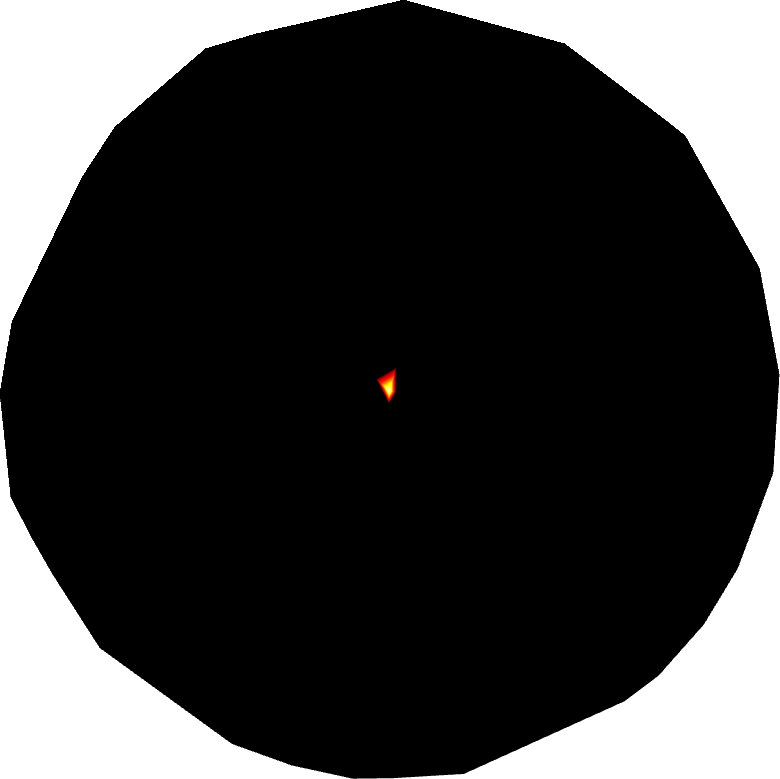
\includegraphics[width=1.0\linewidth,height=0.3\textheight,keepaspectratio]{data/synthetic_meshes/random_circle_tessellation_Dirac_delta_10_v641_f1252_funcvals_0iter.png}
		\caption{R.Circ v641\_f1252 iter 0}\label{fig:rcirc.d}
	\end{subfigure}

	\bigskip
	\begin{subfigure}[b]{0.48\linewidth}
		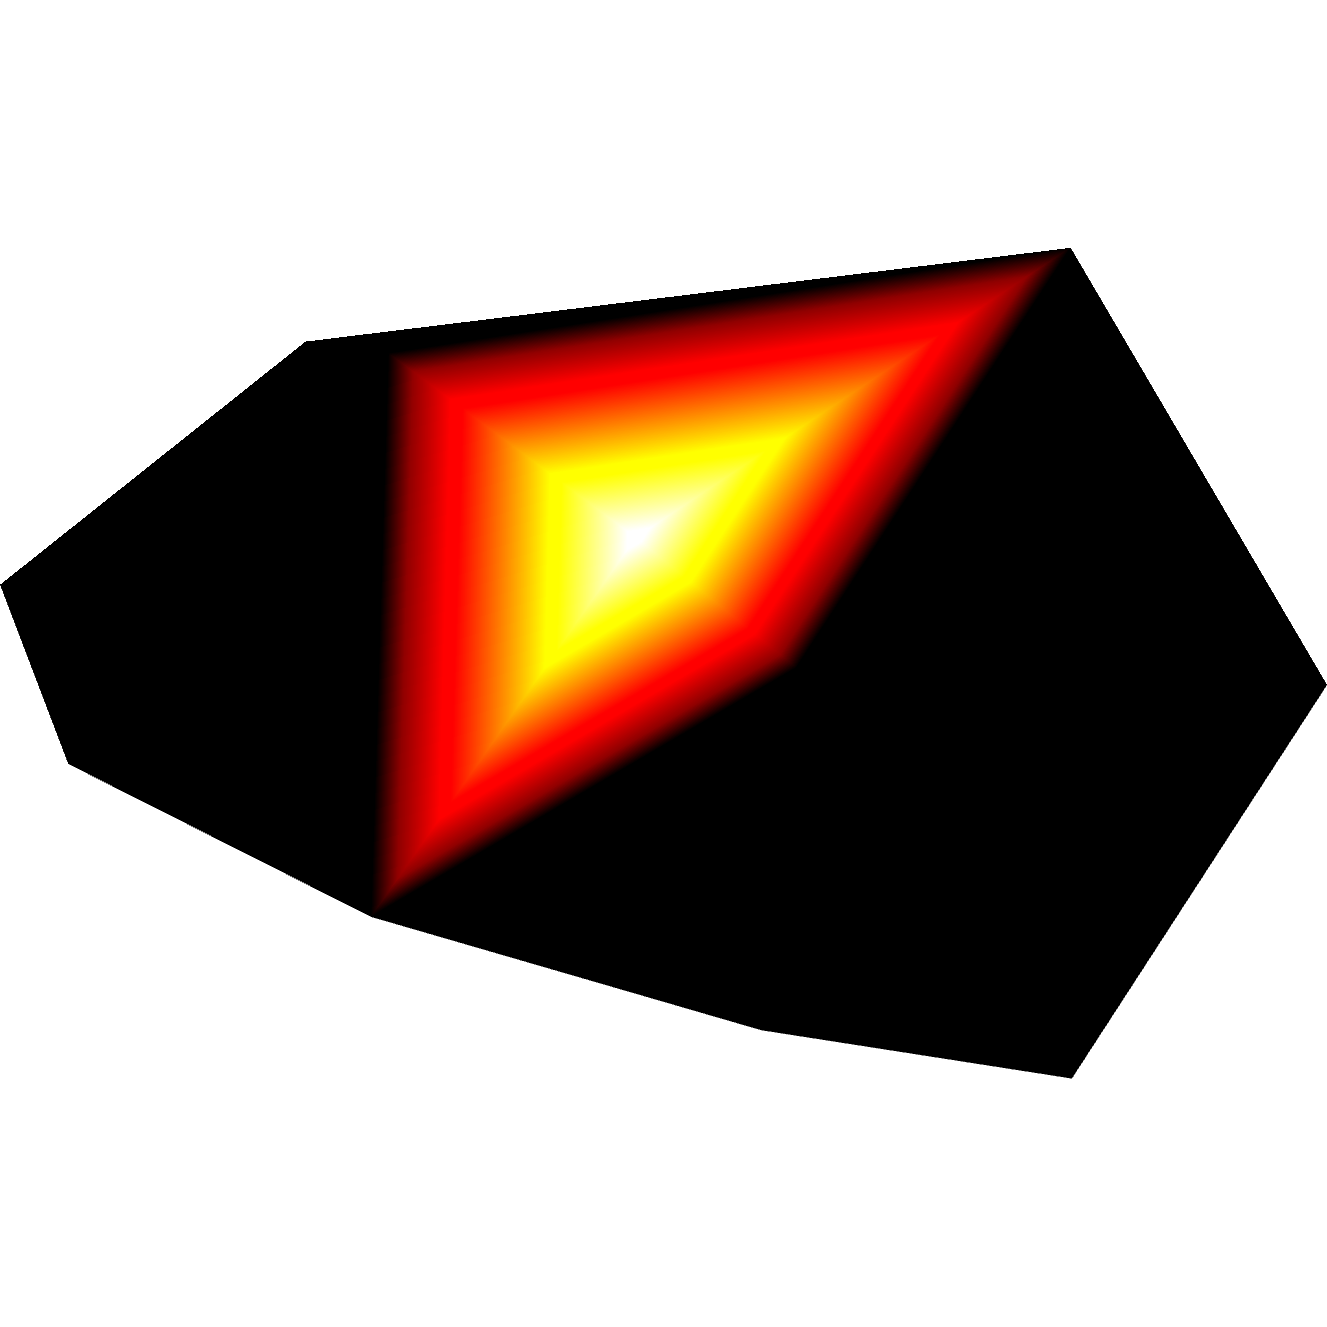
\includegraphics[width=1.0\linewidth,height=0.3\textheight,keepaspectratio,height=0.3\textheight,keepaspectratio]{data/synthetic_meshes/random_circle_tessellation_Dirac_delta_1_v11_f12_funcvals_0iter.png}
		\caption{R.Circ v11\_f12 iter 2}\label{fig:rcirc.e}
	\end{subfigure}
	\begin{subfigure}[b]{0.48\linewidth}
		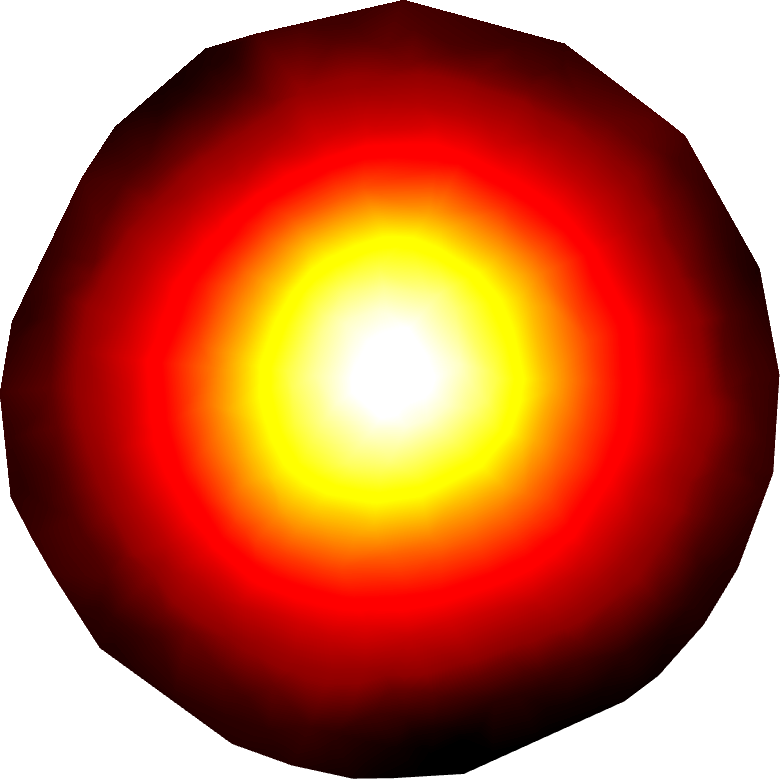
\includegraphics[width=1.0\linewidth,height=0.3\textheight,keepaspectratio,height=0.3\textheight,keepaspectratio]{data/synthetic_meshes/random_circle_tessellation_Dirac_delta_10_v641_f1252_funcvals_10000iter.png}
		\caption{R.Circ v641\_f1252 iter 10,000}\label{fig:rcirc.f}
	\end{subfigure}}
	{\caption[Synthetic random vertices equally distributed per radius, Dirac delta function]{A synthetic circle filled with random vertices equaly distributed per radius, triangulated by Delauney method~\cite[p.~??]{todoCitation}, with a Dirac delta function applied: (a) v11\_f12 wireframe (b) v641\_f1252 wireframe (c) v11\_f12 colored by function value before filter (d) v641\_f1252 colored by function value before filter (e) v11\_f12 colored by function value after 2 iterations (f) v641\_f1252 colored by function value after 10,000 iterations.
%All using the colorramp "Hot (improved)"~\cite[p.~???]{Brewer2003}~\cite[p.~19]{Giga17}, visualized using GigaMesh~\cite{Mara10}, exported as png after disabling the background grid [f7], maximizing the window, disabling screenshot cropping, as well as rejecting tiled rendering, finally cropping to content in GIMP.
}\label{fig:rcirc}}
\end{figure}
\todoCitation{}
\todoResearch{Why and who equally distributed}

%\subsection{Debossed H}
%In Figure \ref{fig:h}, we show a debossed capital letter H.\footnote{The H is
%as a nod to Heidelberg University and the cuniform script studied by the FCGL.}
%\begin{figure}[ht]
%\centering
%	\begin{subfigure}{.48\linewidth}
%		\centering
%		\resizebox{0.48\linewidth}{!}{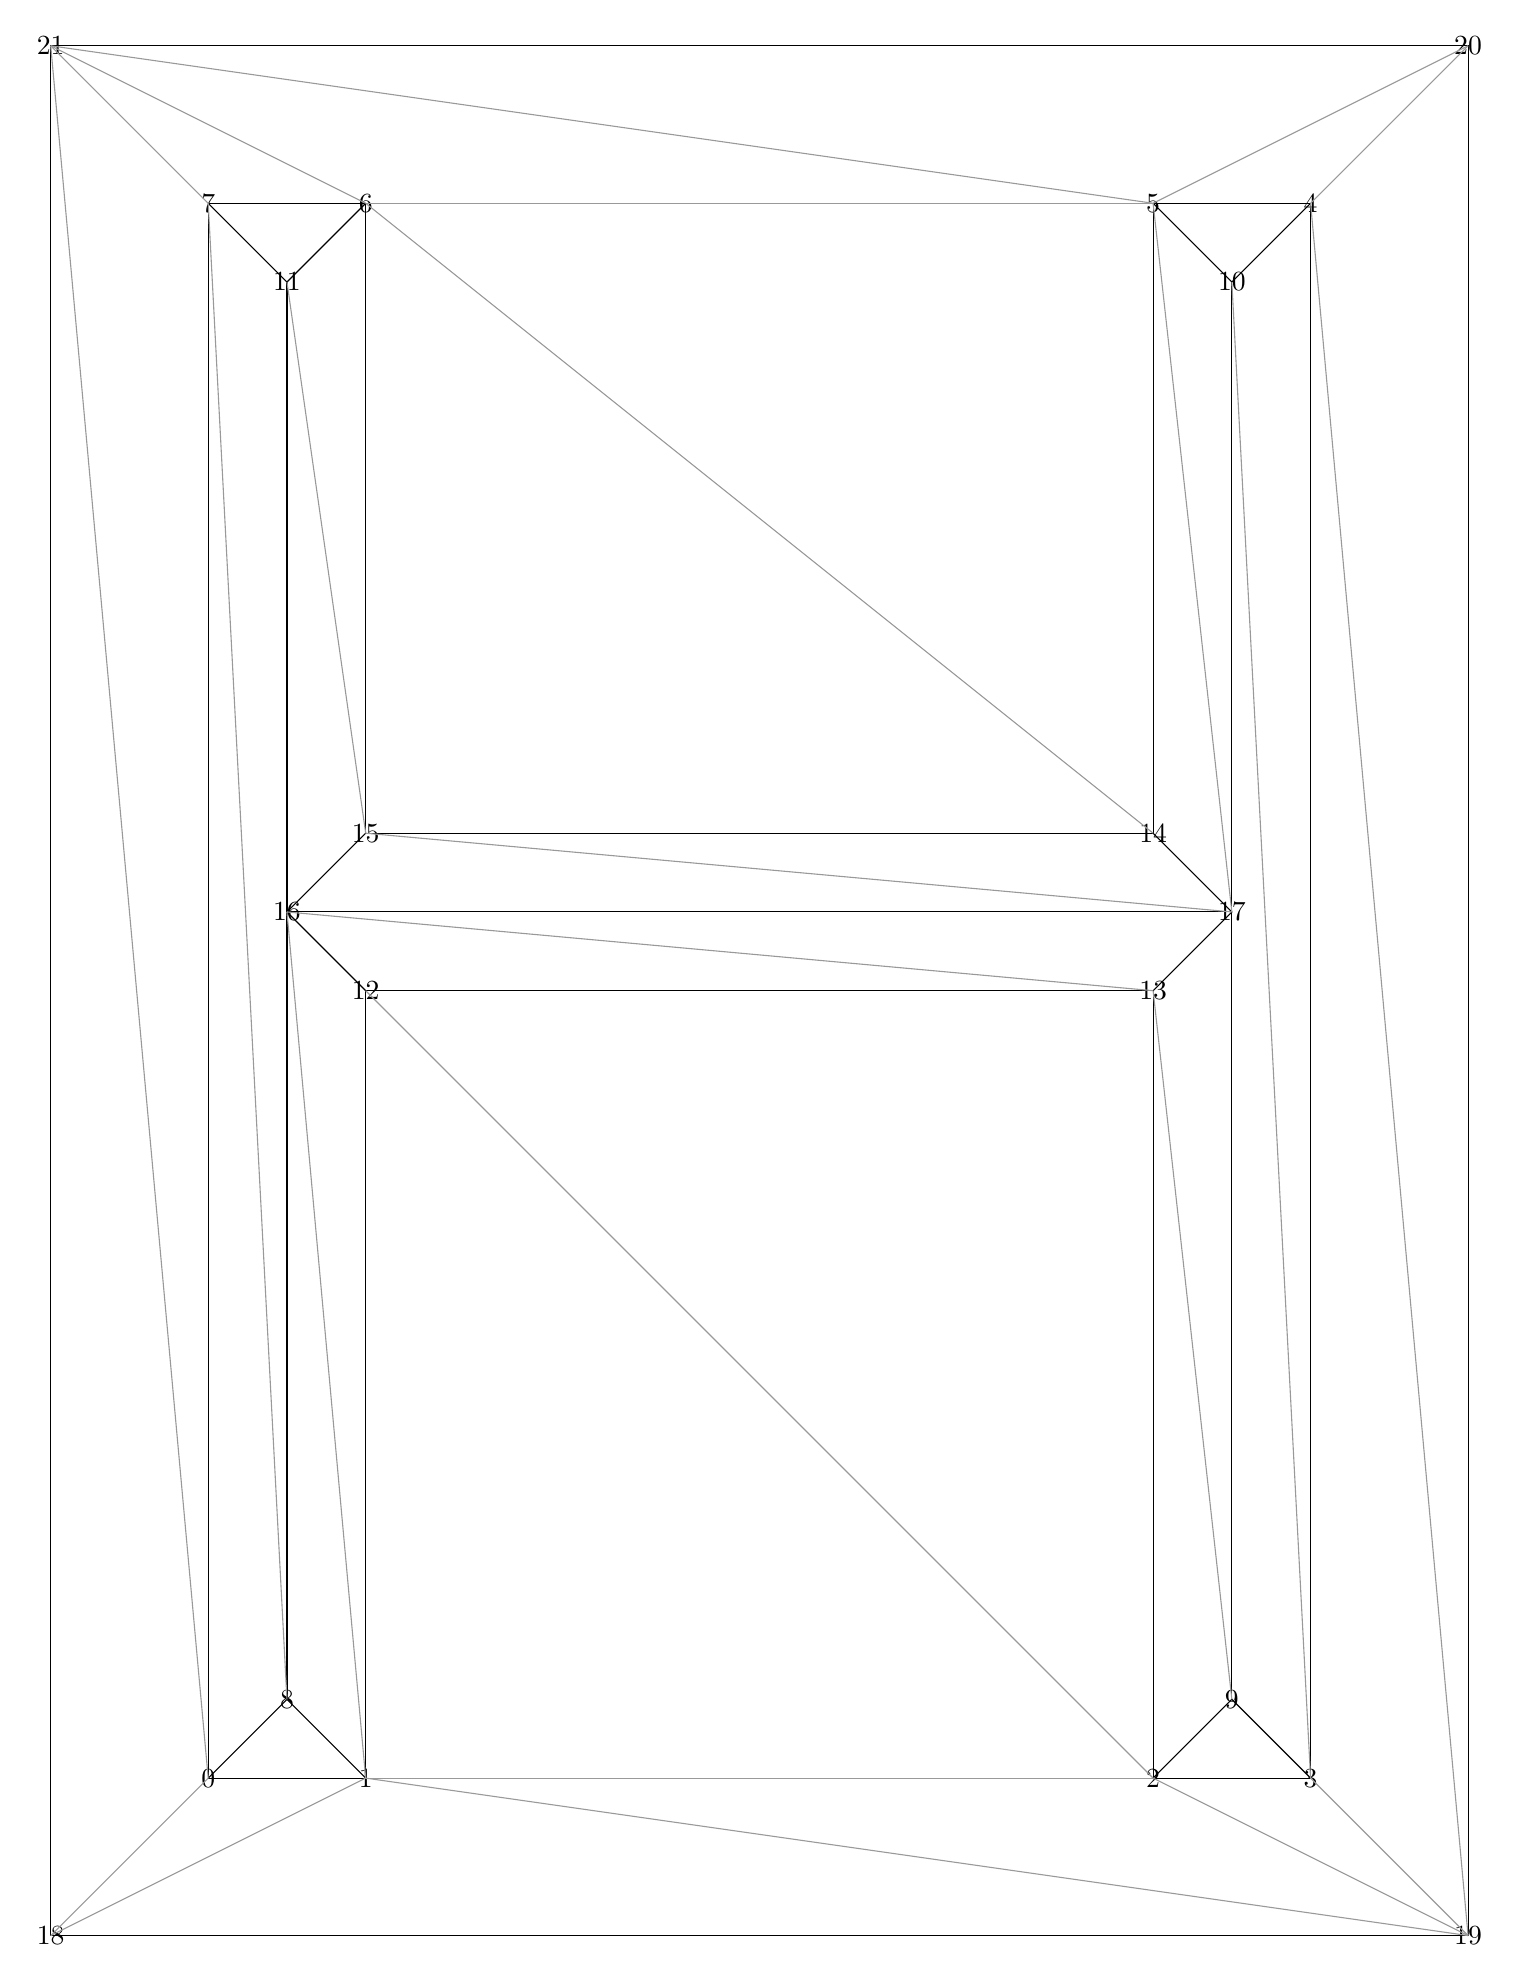
\begin{tikzpicture}
% Colors
\definecolor{outlineColor}{RGB}{0,0,0}
\definecolor{supportColor}{RGB}{153,153,153}
% Main H shape and Outline
\begin{scope}[outlineColor]
	\draw( 0, 0) node  {0} % 0
	  -- ( 2, 0) node  {1} % 1
	  -- ( 2,10) node {12} %12
	  -- (12,10) node {13} %13
	  -- (12, 0) node  {2} % 2
	  -- (14, 0) node  {3} % 3
	  -- (14,20) node  {4} % 4
	  -- (12,20) node  {5} % 5
	  -- (12,12) node {14} %14
	  -- ( 2,12) node {15} %15
	  -- ( 2,20) node  {6} % 6
	  -- ( 0,20) node  {7} % 7
	  -- cycle;  
	\draw( 0, 0) % 0
	  -- ( 1, 1) node  {8} % 8
	  -- ( 2, 0);% 1
	\draw(12, 0) % 2
	  -- (13, 1) node  {9} % 9
	  -- (14, 0);% 3
	\draw(14,20) % 4
	  -- (13,19) node {10} %10
	  -- (12,20);% 5
	\draw( 2,20) % 6
	  -- ( 1,19) node {11} %11
	  -- ( 0,20);% 7
	\draw( 2,10) %12
	  -- ( 1,11) node {16} %16
	  -- ( 2,12);%15
	\draw(12,10) %13
	  -- (13,11) node {17} %17
	  -- (12,12);%14
	\draw( 1, 1) % 8
	  -- ( 1,19);%11
	\draw(13, 1) % 9
	  -- (13,19);%10
	\draw( 1,11) %16
	  -- (13,11);%17
	\draw(-2,-2) node {18} %18
	  -- (16,-2) node {19} %19
	  -- (16,22) node {20} %20
	  -- (-2,22) node {21} %21
	  -- cycle;
\end{scope}
\begin{scope}[supportColor, thin]
	\draw( 0, 0) -- (-2,-2); % 0--18
	\draw( 0, 0) -- (-2,22); % 0--21
	\draw( 2, 0) -- (12, 0); % 1-- 2
	\draw( 2, 0) -- ( 1,11); % 1--16
	\draw( 2, 0) -- (-2,-2); % 1--18
	\draw( 2, 0) -- (16,-2); % 1--19
	\draw(12, 0) -- ( 2,10); % 2--12
	\draw(12, 0) -- (16,-2); % 2--19
	\draw(14, 0) -- (13,19); % 3--10
	\draw(14, 0) -- (16,-2); % 3--19
	\draw(14,20) -- (16,-2); % 4--19
	\draw(14,20) -- (16,22); % 4--20
	\draw(12,20) -- ( 2,20); % 5-- 6
	\draw(12,20) -- (13,11); % 5--17
	\draw(12,20) -- (16,22); % 5--20
	\draw(12,20) -- (-2,22); % 5--21
	\draw( 2,20) -- (12,12); % 6--14
	\draw( 2,20) -- (-2,22); % 6--21
	\draw( 0,20) -- ( 1, 1); % 7-- 8
	\draw( 0,20) -- (-2,22); % 7--21
	\draw(13, 1) -- (12,10); % 9--13
	\draw( 1,19) -- ( 2,12); %11--15
	\draw(12,10) -- ( 1,11); %13--16
	\draw( 2,12) -- (13,11); %15--17
\end{scope}
\end{tikzpicture}
}
%		\caption{HWireframe}\label{fig:h.a}
%	\end{subfigure}
%	\hfill
%	\begin{subfigure}{.48\linewidth}
%		\centering
%		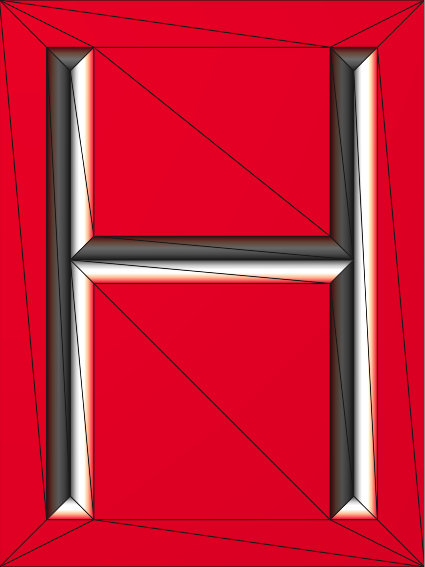
\includegraphics[width=0.48\linewidth]{data/synthetic_meshes/h_colored.png}
%		\caption{HColored}\label{fig:h.b}
%	\end{subfigure}
%	\caption[A debossed H, which contains 22 vertices and 36 faces.]{A debossed H,
%	which contains 22 vertices and 36 faces: (a) wireframe (b) colored by the
%	relation to its distance to an underlying plane, in RdGy
%	colorramp~\cite[p.~???]{Brewer2003}~\cite[p.~19]{Giga17}, visualized using the
%	GigaMesh~\cite{Mara10} framework with triangle edges rendered.}\label{fig:h}
%\end{figure}
To evaluate methods available for discrete surfaces, we can increase the number
of vertices of our synthetic wedge using five iterations of the mid-edge
subdivision scheme [PR97,
HW99].~\cite[p.~38]{Mara12}



\section{Acquired Data}
Acquired Data examples are actually recorded by sensors.
Something in Archaeology
Cuneiform Tablets
Mayan Tablets
Dynamic Earth models

\subsection{University Seal}
Unisiegel\_\- UAH\_\- Ebay-Siegel\_\- Uniarchiv\_\- HE2066-60\_\- 010614\_\- partial\_\- ASCII.ply
%\begin{figure}[ht]
%\ffigbox
%	{\begin{subfigure}[b]{0.48\linewidth}
%		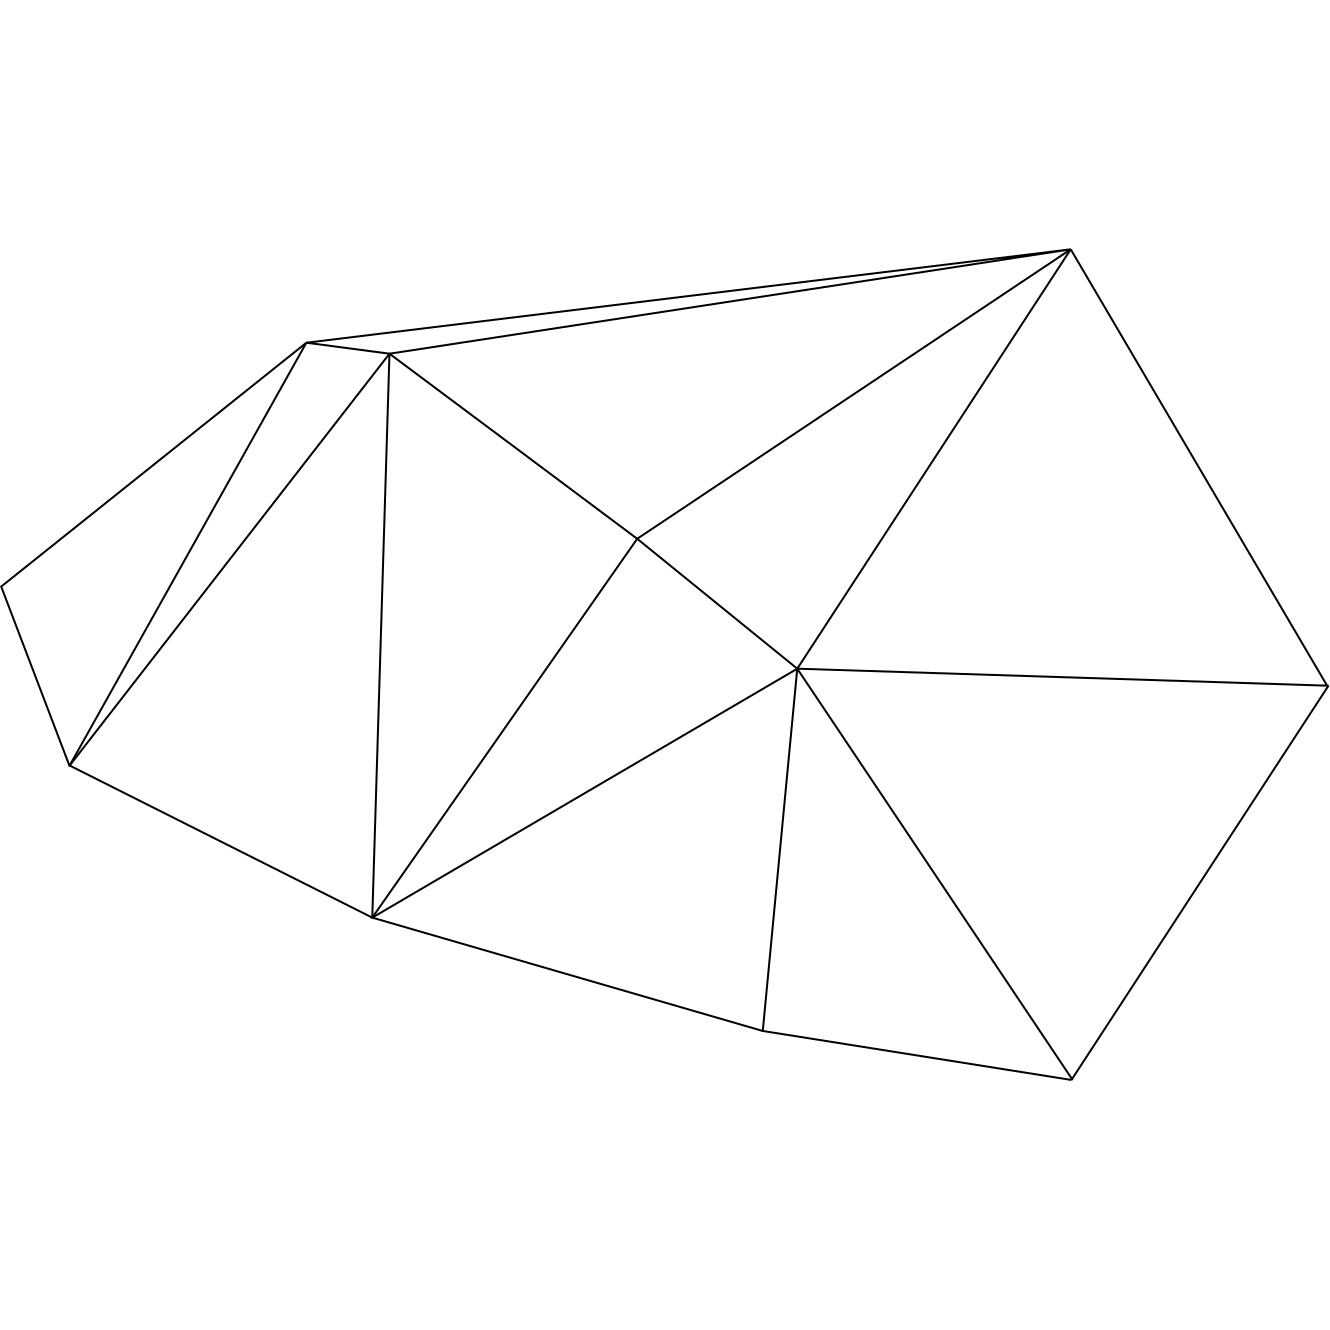
\includegraphics[width=1.0\linewidth,height=0.3\textheight,keepaspectratio]{data/synthetic_meshes/random_circle_tessellation_Dirac_delta_1_v11_f12_wireframe.png}
%		\caption{R.Circ v11\_f12 wireframe}\label{fig:rcirc.a}
%	\end{subfigure}
%	\begin{subfigure}[b]{0.48\linewidth}
%		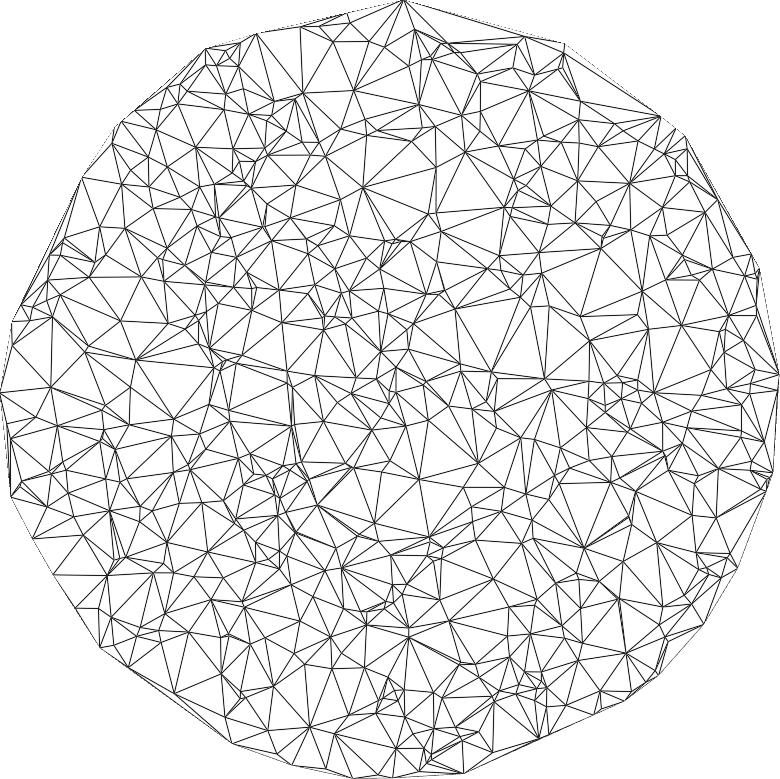
\includegraphics[width=1.0\linewidth,height=0.3\textheight,keepaspectratio]{data/synthetic_meshes/random_circle_tessellation_Dirac_delta_10_v641_f1252_wireframe.png}
%		\caption{R.Circ v641\_f1252 wireframe}\label{fig:rcirc.b}
%	\end{subfigure}
%
%	\bigskip
%	\begin{subfigure}[b]{0.48\linewidth}
%		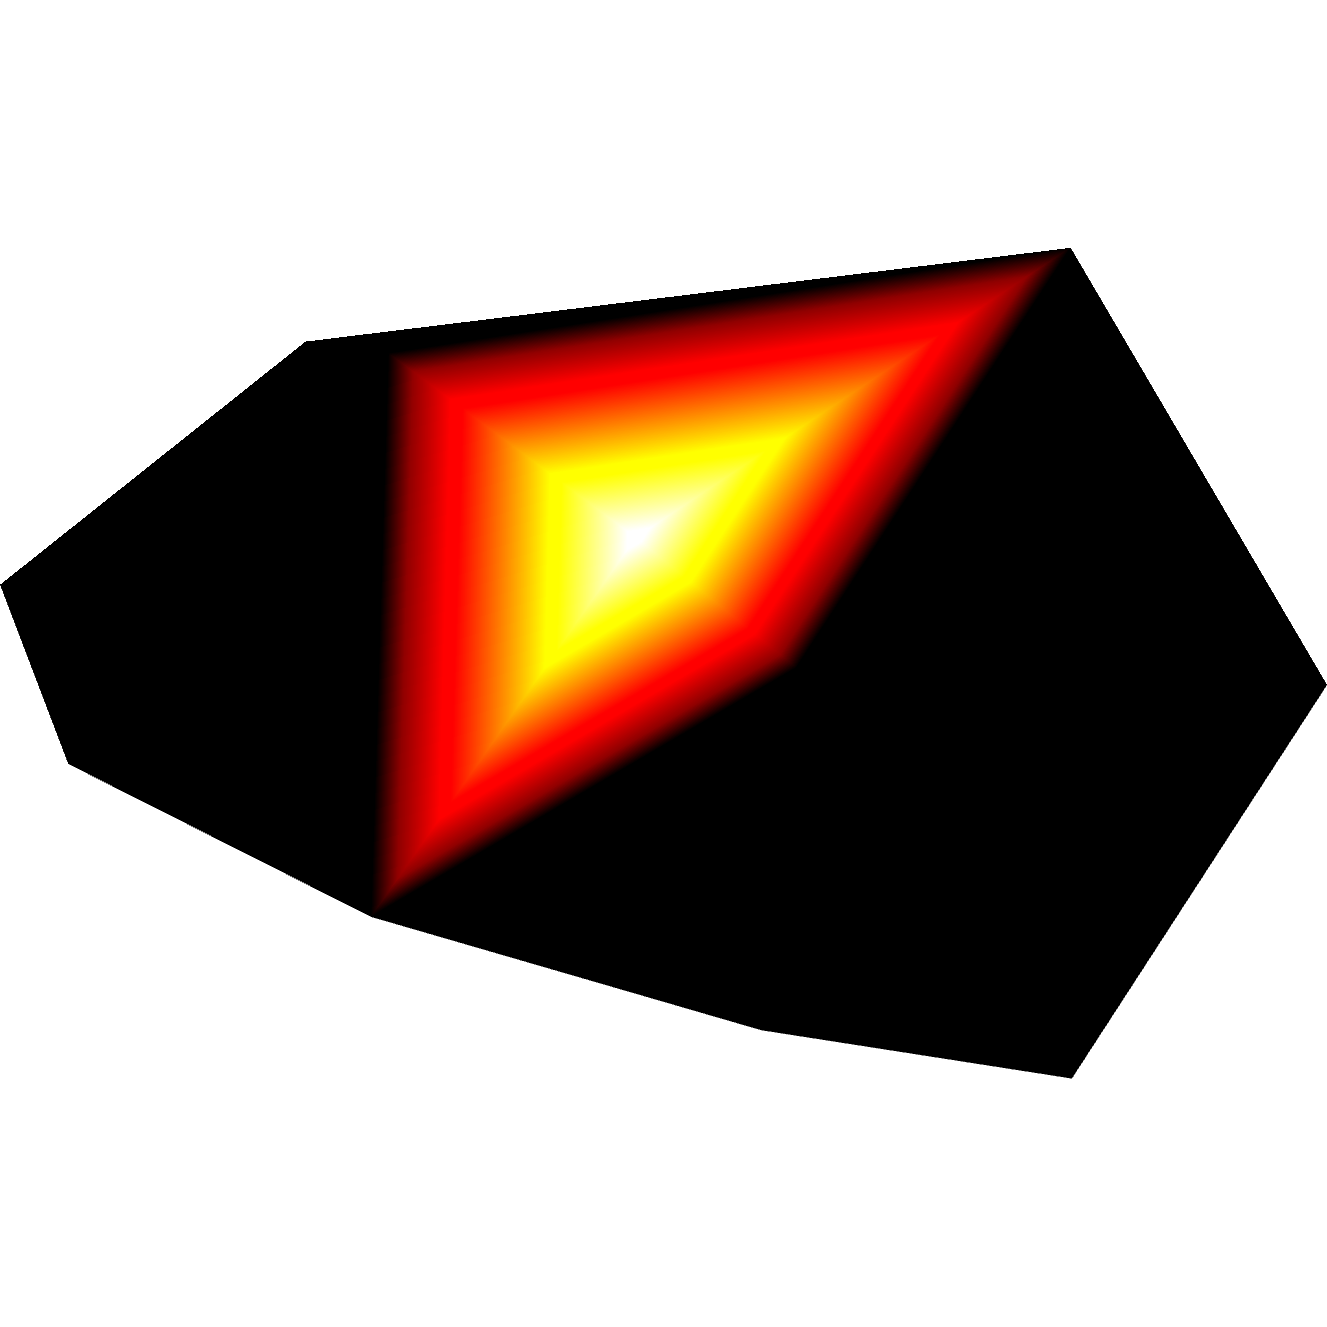
\includegraphics[width=1.0\linewidth,height=0.3\textheight,keepaspectratio]{data/synthetic_meshes/random_circle_tessellation_Dirac_delta_1_v11_f12_funcvals_0iter.png}
%		\caption{R.Circ v11\_f12 iter 0}\label{fig:rcirc.c}
%	\end{subfigure}
%	\begin{subfigure}[b]{0.48\linewidth}
%		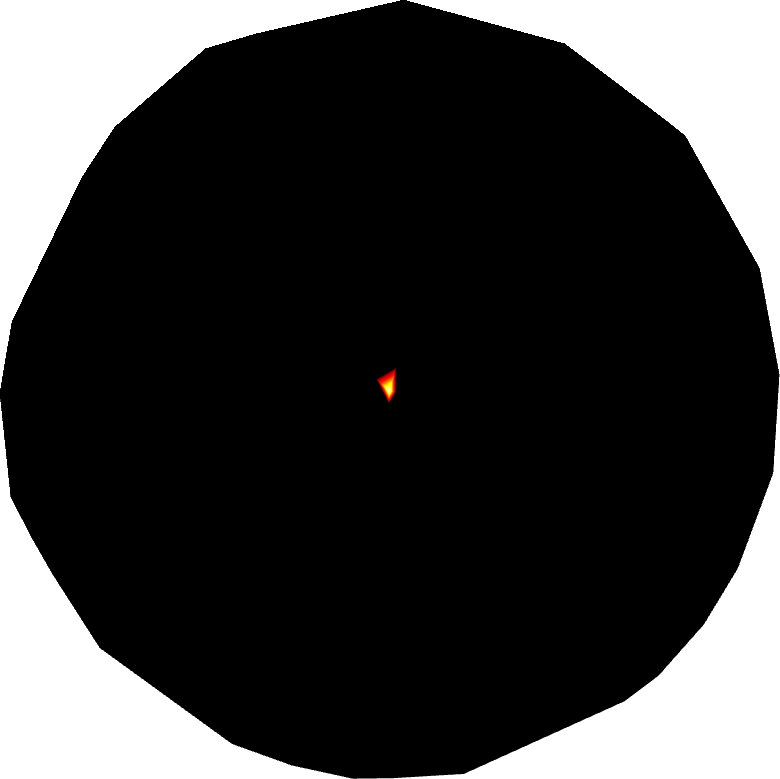
\includegraphics[width=1.0\linewidth,height=0.3\textheight,keepaspectratio]{data/synthetic_meshes/random_circle_tessellation_Dirac_delta_10_v641_f1252_funcvals_0iter.png}
%		\caption{R.Circ v641\_f1252 iter 0}\label{fig:rcirc.d}
%	\end{subfigure}
%
%	\bigskip
%	\begin{subfigure}[b]{0.48\linewidth}
%		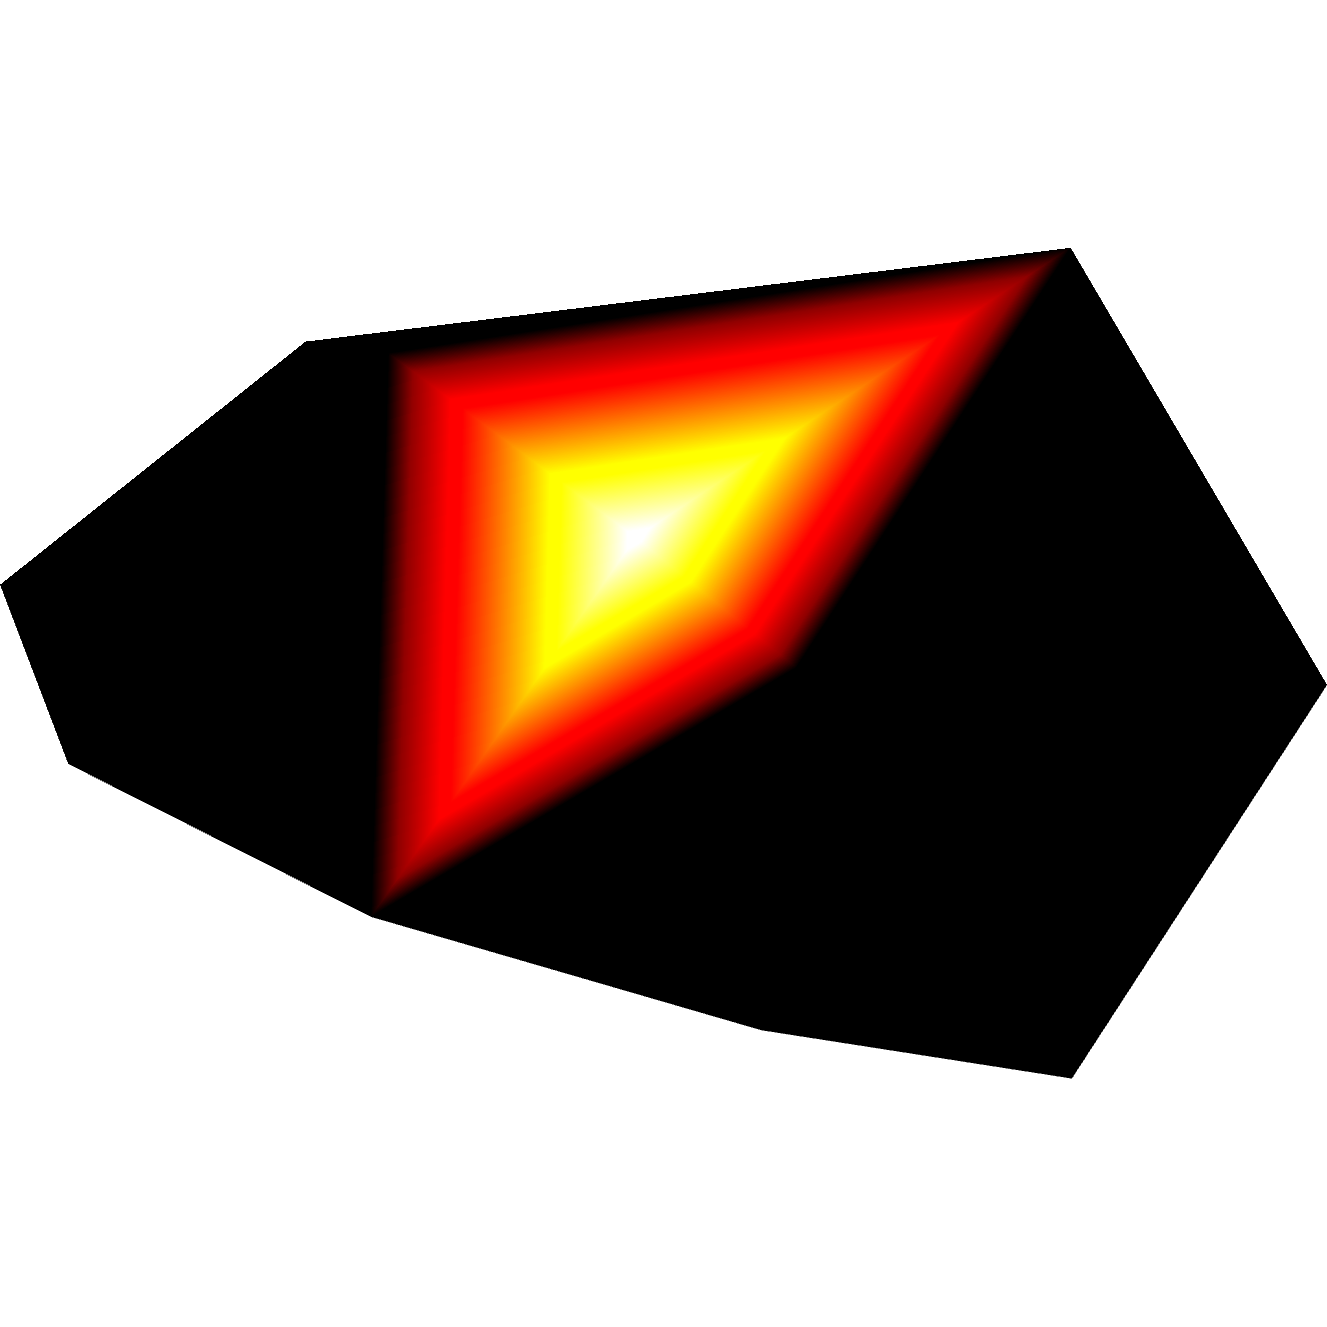
\includegraphics[width=1.0\linewidth,height=0.3\textheight,keepaspectratio]{data/synthetic_meshes/random_circle_tessellation_Dirac_delta_1_v11_f12_funcvals_0iter.png}
%		\caption{R.Circ v11\_f12 iter 2}\label{fig:rcirc.e}
%	\end{subfigure}
%	\begin{subfigure}[b]{0.48\linewidth}
%		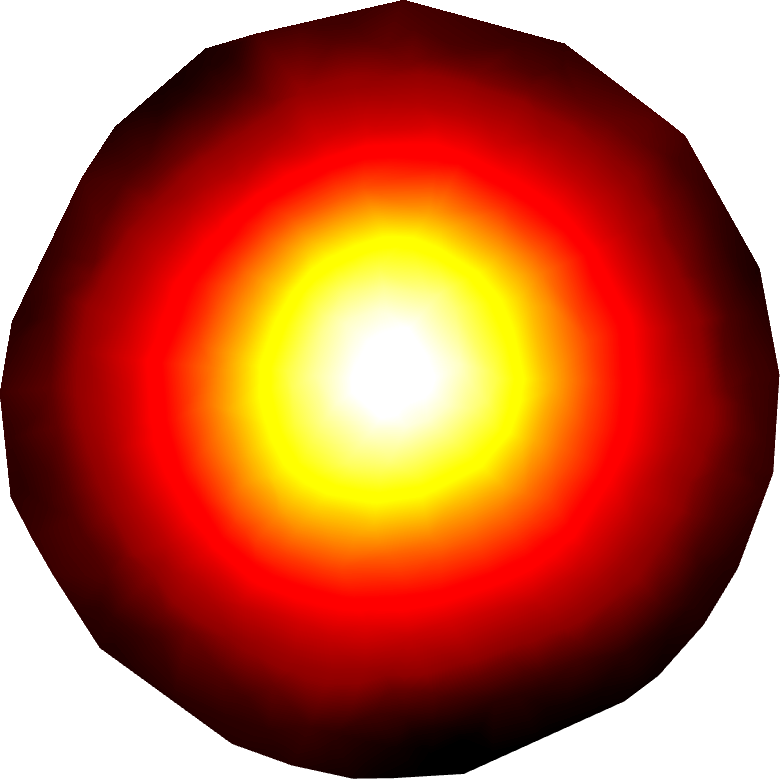
\includegraphics[width=1.0\linewidth,height=0.3\textheight,keepaspectratio]{data/synthetic_meshes/random_circle_tessellation_Dirac_delta_10_v641_f1252_funcvals_10000iter.png}
%		\caption{R.Circ v641\_f1252 iter 10,000}\label{fig:rcirc.f}
%	\end{subfigure}}
%	{\caption[Synthetic random vertices equally distributed per radius, Dirac delta function]{A synthetic circle filled with random vertices equaly distributed per radius, triangulated by Delauney method~\cite[p.~??]{todoCitation}, with a Dirac delta function applied: (a) v11\_f12 wireframe (b) v641\_f1252 wireframe (c) v11\_f12 colored by function value before filter (d) v641\_f1252 colored by function value before filter (e) v11\_f12 colored by function value after 2 iterations (f) v641\_f1252 colored by function value after 10,000 iterations.
%All using the colorramp "Hot (improved)"~\cite[p.~???]{Brewer2003}~\cite[p.~19]{Giga17}, visualized using GigaMesh~\cite{Mara10}, exported as png after disabling the background grid [f7], maximizing the window, disabling screenshot cropping, as well as rejecting tiled rendering, finally cropping to content in GIMP.
%}\label{fig:rcirc}}
%\end{figure}

\subsection{Mars Crater}
Mars dataset crater as a Digital Terrain Models (DTMs) Mention in Mara 3.6
Summary “Dali” inspired methodProcessing regular grids like Digital Terrain
Models (DTMs) will gain dramatic performance increases using the estimator,
while processing irregular grids with high curvatures will strongly benefit
from precise computation of the volume integral invariant.~\cite[p.~143]{Mara12}

\subsection{A Flat surface}
Flat surfaces have NOISE!
Figure~\ref{fig:ILATO}: ILATO\_1A\_SM2066-HE5-60\_070214\_merged\_GMO\_r1.00\_n4\_v256
\begin{figure}[ht]
\ffigbox
	{\begin{subfigure}[b]{0.48\linewidth}
		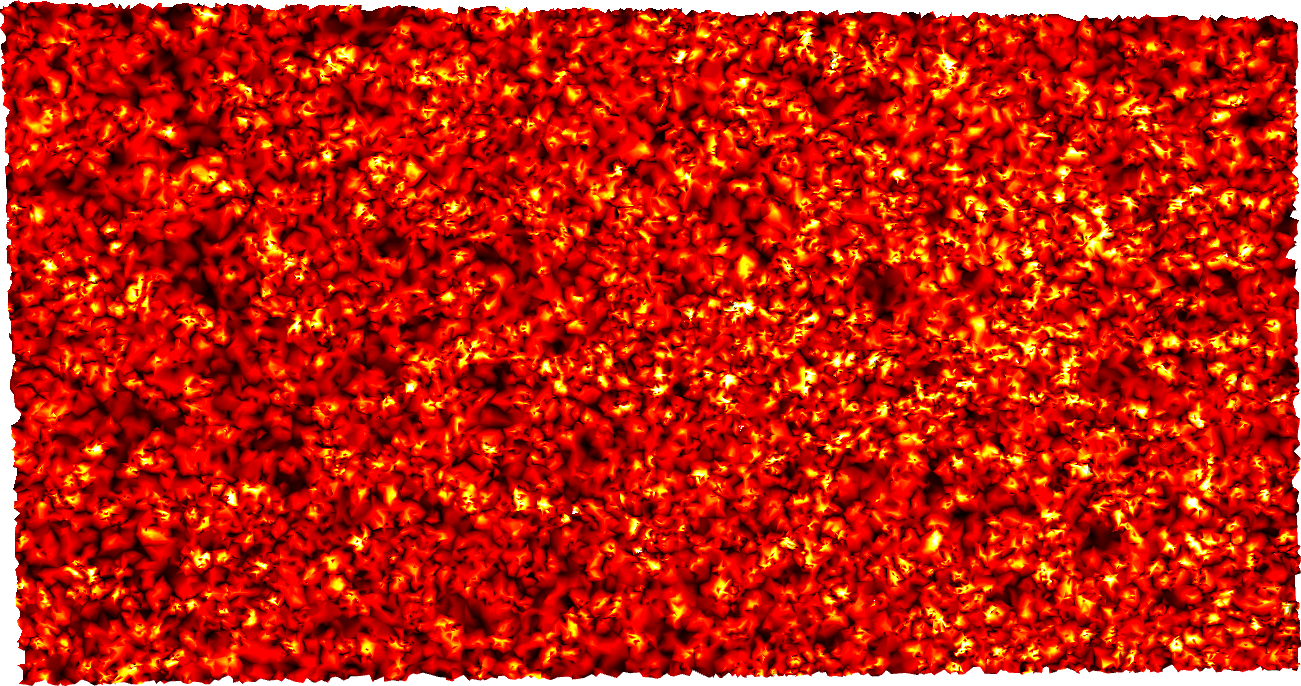
\includegraphics[width=1.0\linewidth,height=0.3\textheight,keepaspectratio]{data/acquired_meshes/ILATO_1A_SM2066-HE5-60_070214_merged_GMO_r1_n4_v256_funcvals_0iter.png}
		\caption{ILATO 0iter}\label{fig:ILATO.a}
	\end{subfigure}
	\begin{subfigure}[b]{0.48\linewidth}
		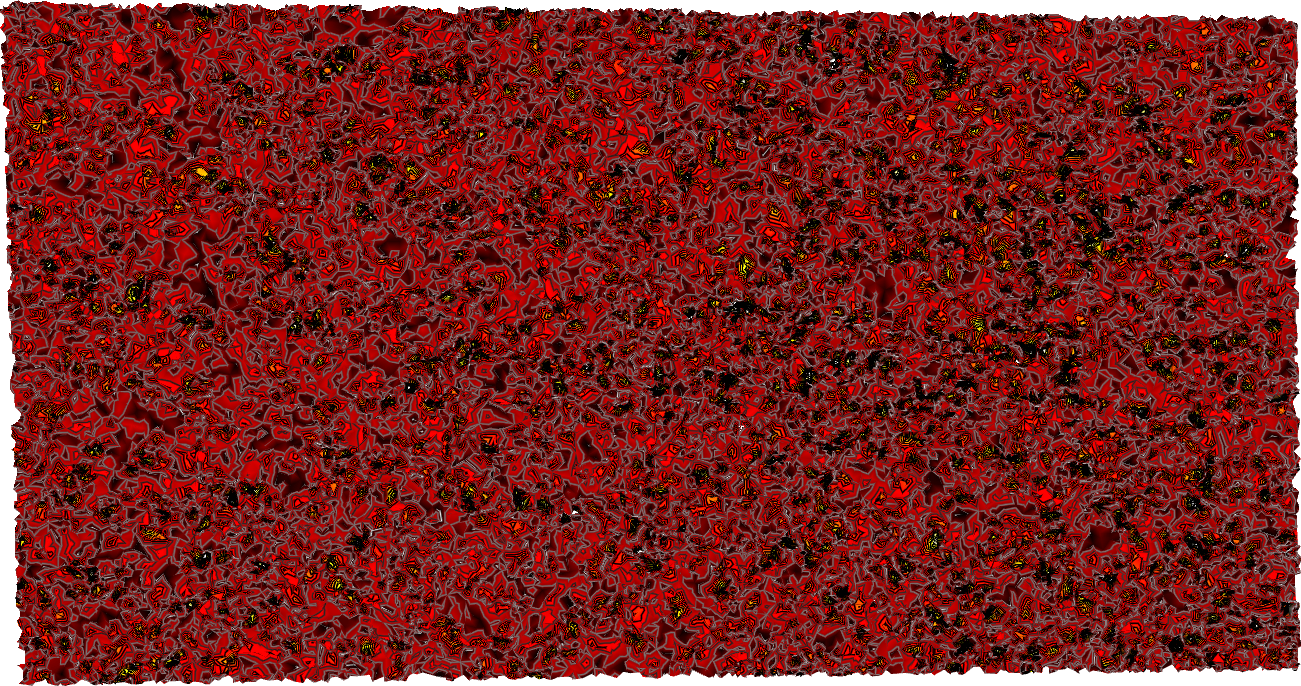
\includegraphics[width=1.0\linewidth,height=0.3\textheight,keepaspectratio]{data/acquired_meshes/ILATO_1A_SM2066-HE5-60_070214_merged_GMO_r1_n4_v256_funcvals_isolines_0iter.png}
		\caption{ILATO 0iter isolines}\label{fig:ILATO.b}
	\end{subfigure}

	\bigskip
	\begin{subfigure}[b]{0.48\linewidth}
		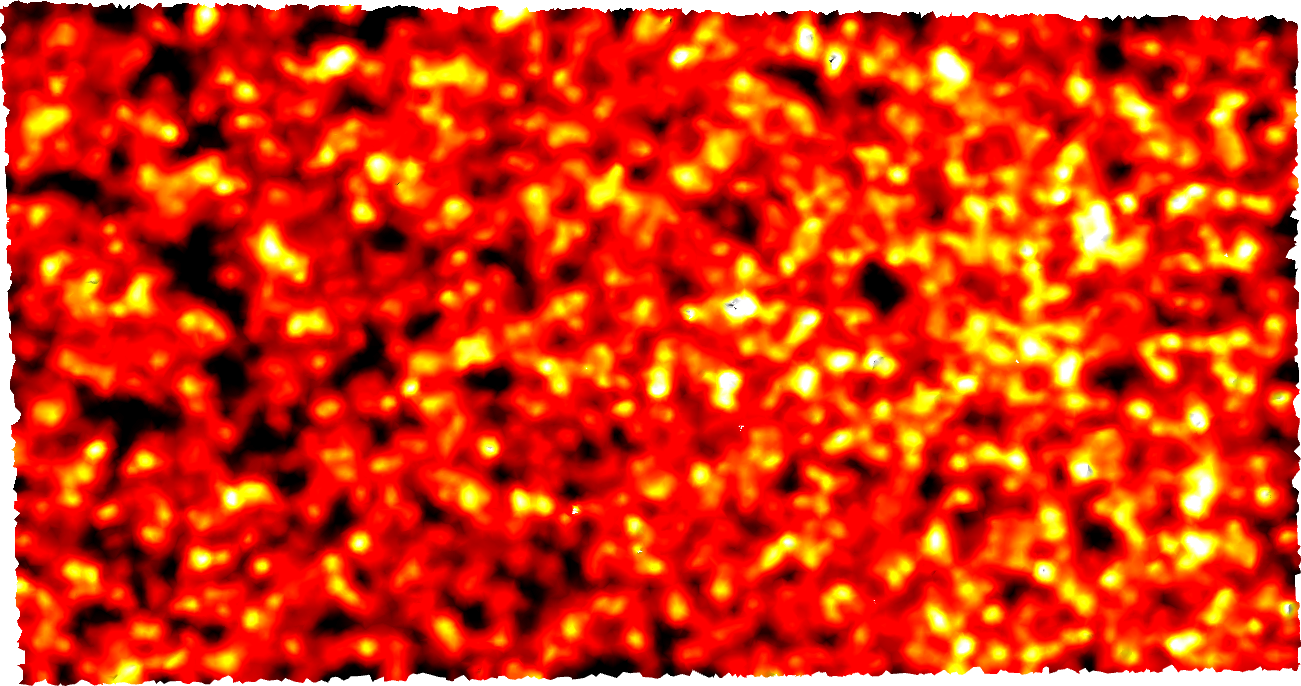
\includegraphics[width=1.0\linewidth,height=0.3\textheight,keepaspectratio]{data/acquired_meshes/ILATO_1A_SM2066-HE5-60_070214_merged_GMO_r1_n4_v256_funcvals_1000iter.png}
		\caption{ILATO 1000iter}\label{fig:ILATO.c}
	\end{subfigure}
	\begin{subfigure}[b]{0.48\linewidth}
		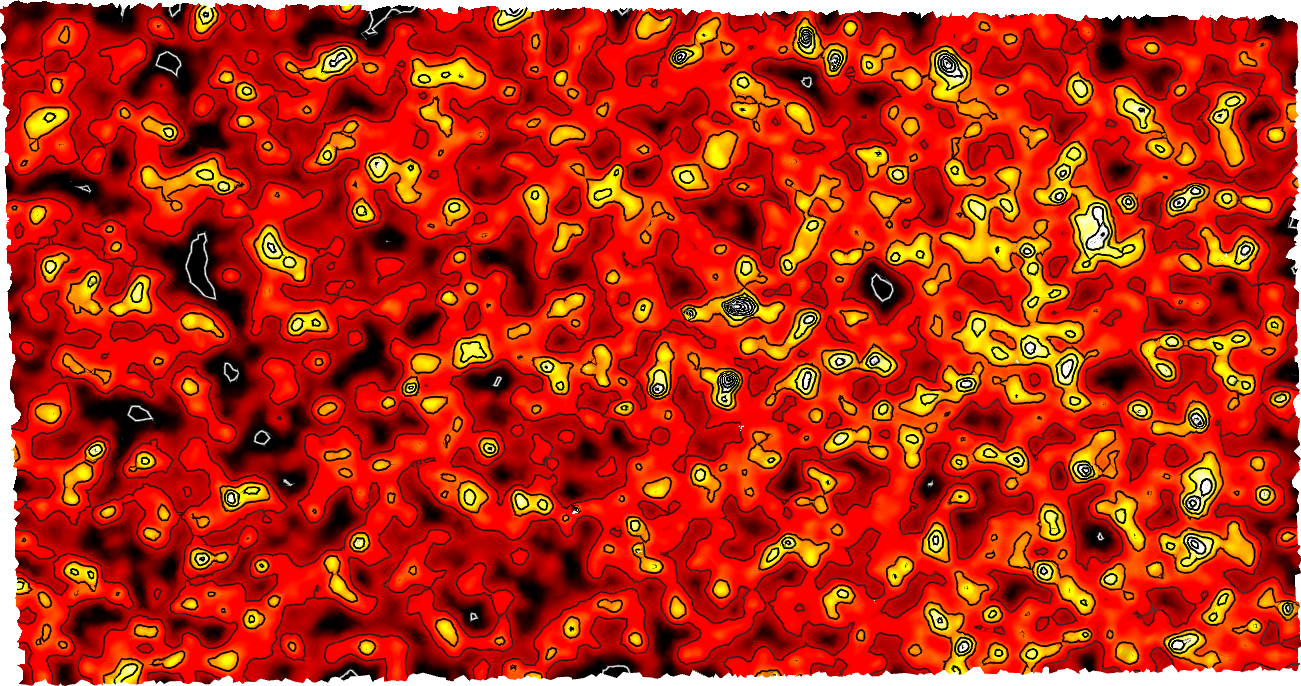
\includegraphics[width=1.0\linewidth,height=0.3\textheight,keepaspectratio]{data/acquired_meshes/ILATO_1A_SM2066-HE5-60_070214_merged_GMO_r1_n4_v256_funcvals_isolines_1000iter.png}
		\caption{ILATO 1000iter isolines}\label{fig:ILATO.d}
	\end{subfigure}

	\bigskip
	\begin{subfigure}[b]{0.48\linewidth}
		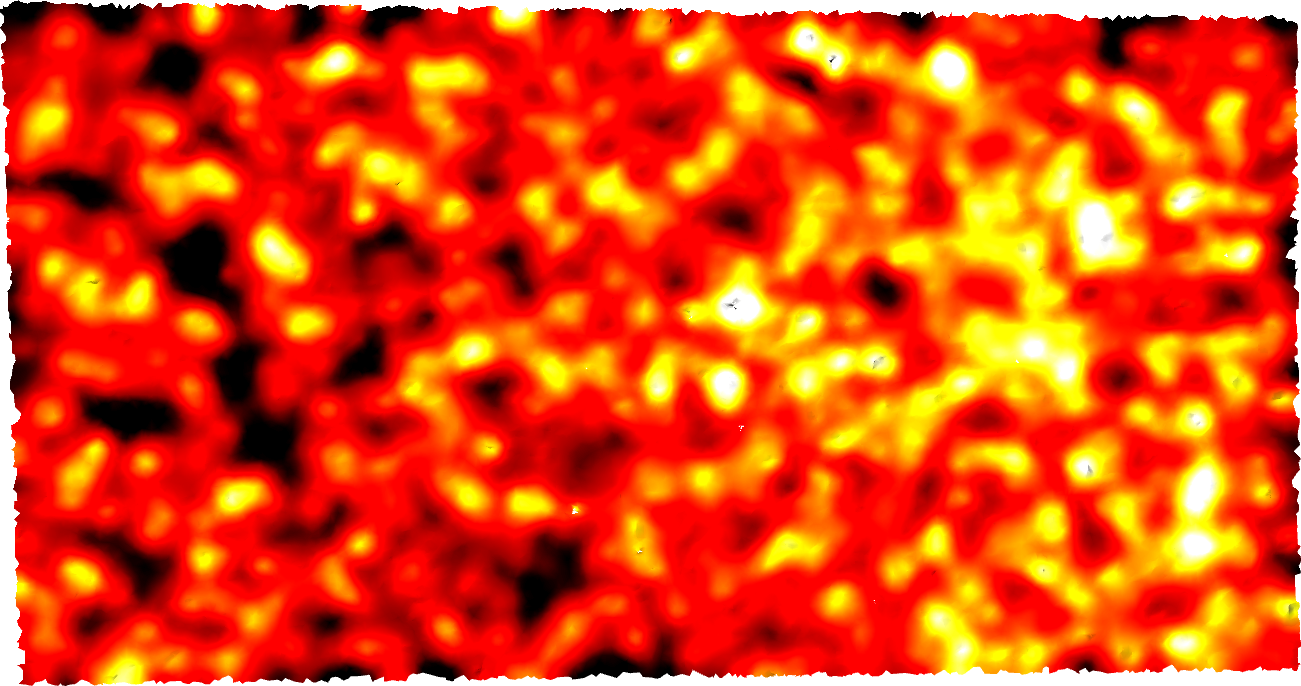
\includegraphics[width=1.0\linewidth,height=0.3\textheight,keepaspectratio]{data/acquired_meshes/ILATO_1A_SM2066-HE5-60_070214_merged_GMO_r1_n4_v256_funcvals_3000iter.png}
		\caption{ILATO 3000iter}\label{fig:ILATO.e}
	\end{subfigure}
	\begin{subfigure}[b]{0.48\linewidth}
		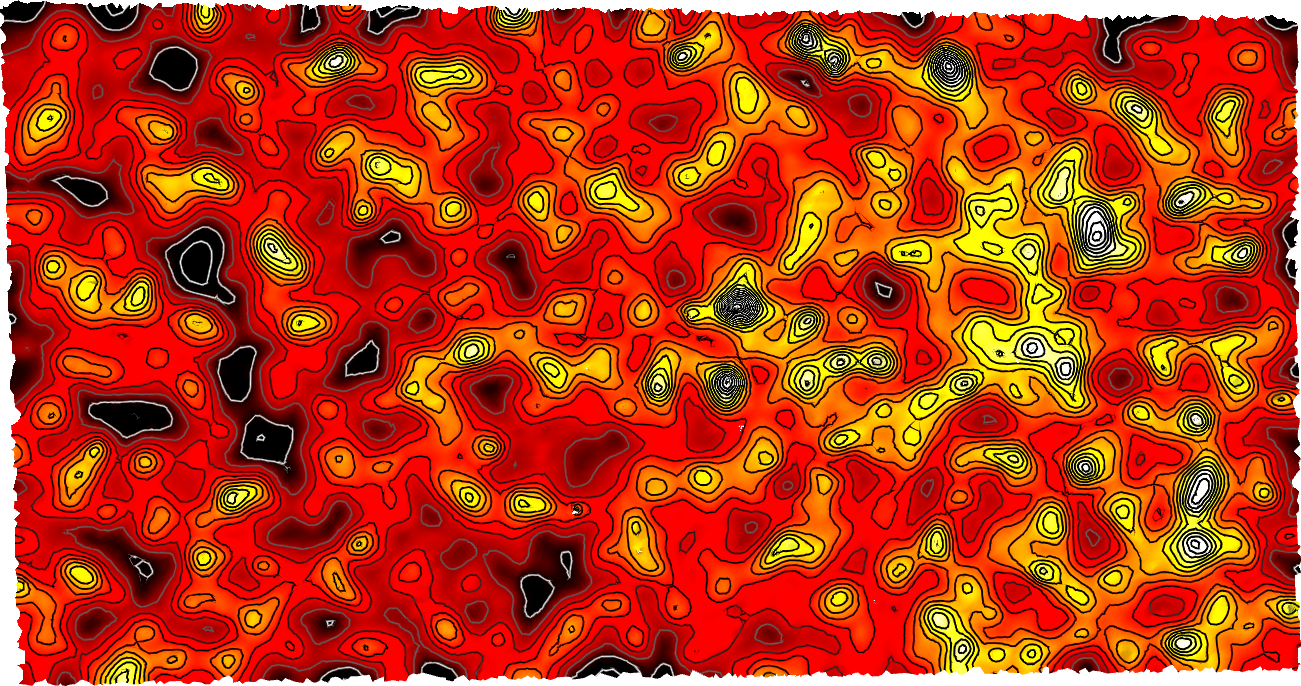
\includegraphics[width=1.0\linewidth,height=0.3\textheight,keepaspectratio]{data/acquired_meshes/ILATO_1A_SM2066-HE5-60_070214_merged_GMO_r1_n4_v256_funcvals_isolines_3000iter.png}
		\caption{ILATO 3000iter isolines}\label{fig:ILATO.f}
	\end{subfigure}}
	{\caption[ILATO]{ILATO\_1A\ldots}\label{fig:ILATO}}
\end{figure}

\subsection{Stanford Bunny}
Figure~\ref{fig:bun}: http://graphics.stanford.edu/data/3Dscanrep/ (Stanford Bunny)
\begin{figure}[ht]
\ffigbox
	{\begin{subfigure}[b]{0.48\linewidth}
		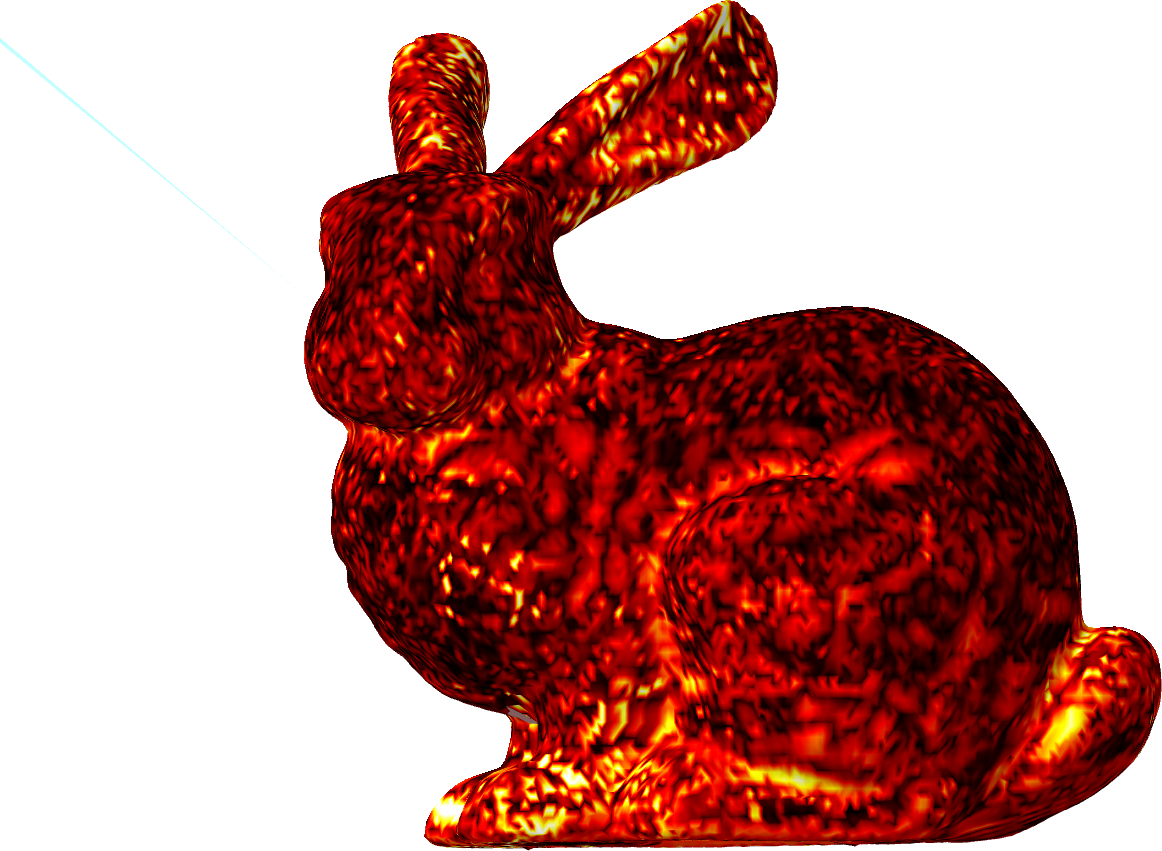
\includegraphics[width=1.0\linewidth,height=0.3\textheight,keepaspectratio]{data/acquired_meshes/bun_zipper_edited_r1_n4_v256_funcvals_0iter.png}
		\caption{Stanford Bunny 0iter}\label{fig:bun.a}
	\end{subfigure}
	\begin{subfigure}[b]{0.48\linewidth}
		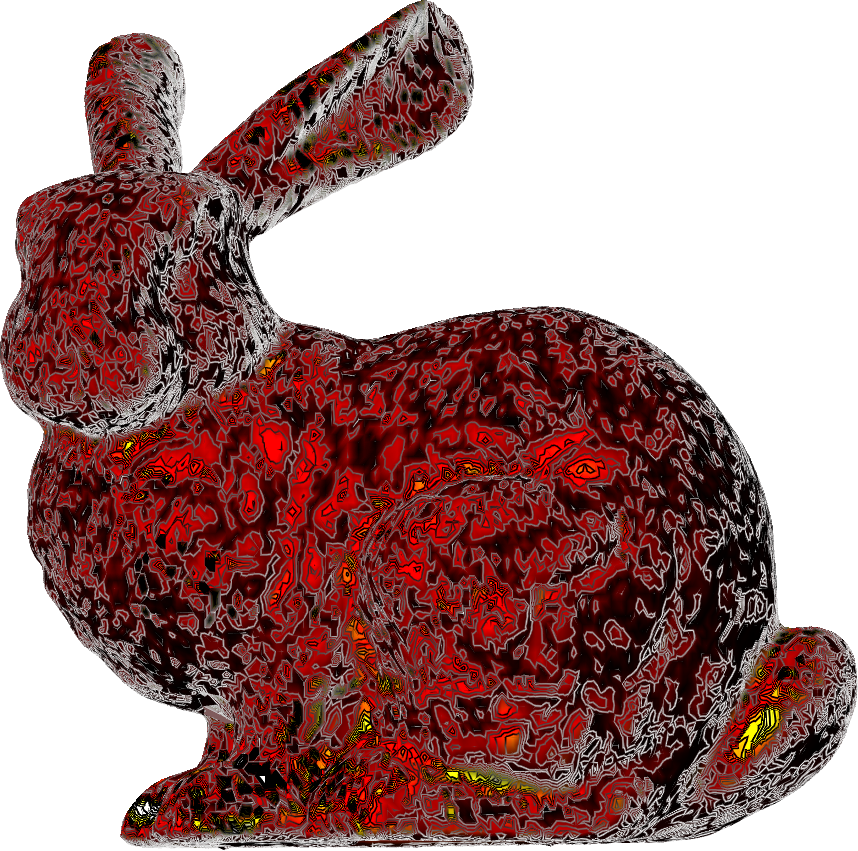
\includegraphics[width=1.0\linewidth,height=0.3\textheight,keepaspectratio]{data/acquired_meshes/bun_zipper_edited_r1_n4_v256_funcvals_isolines_0iter.png}
		\caption{Stanford Bunny 0iter isolines}\label{fig:bun.b}
	\end{subfigure}

	\bigskip
	\begin{subfigure}[b]{0.48\linewidth}
		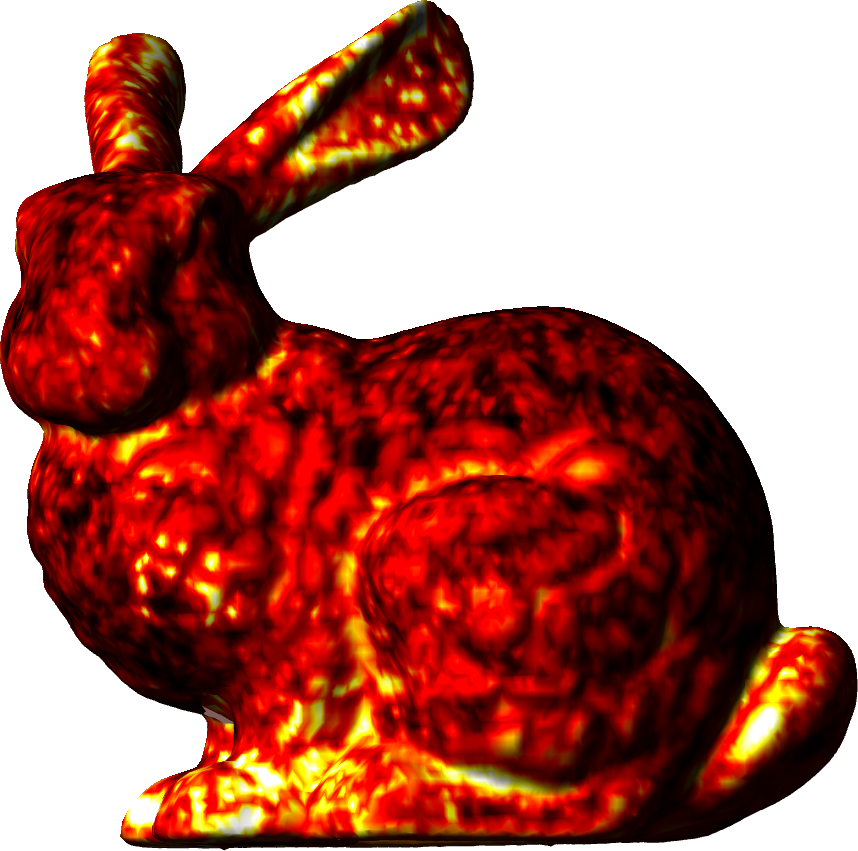
\includegraphics[width=1.0\linewidth,height=0.3\textheight,keepaspectratio]{data/acquired_meshes/bun_zipper_edited_r1_n4_v256_funcvals_10iter.png}
		\caption{Stanford Bunny 10iter}\label{fig:bun.c}
	\end{subfigure}
	\begin{subfigure}[b]{0.48\linewidth}
		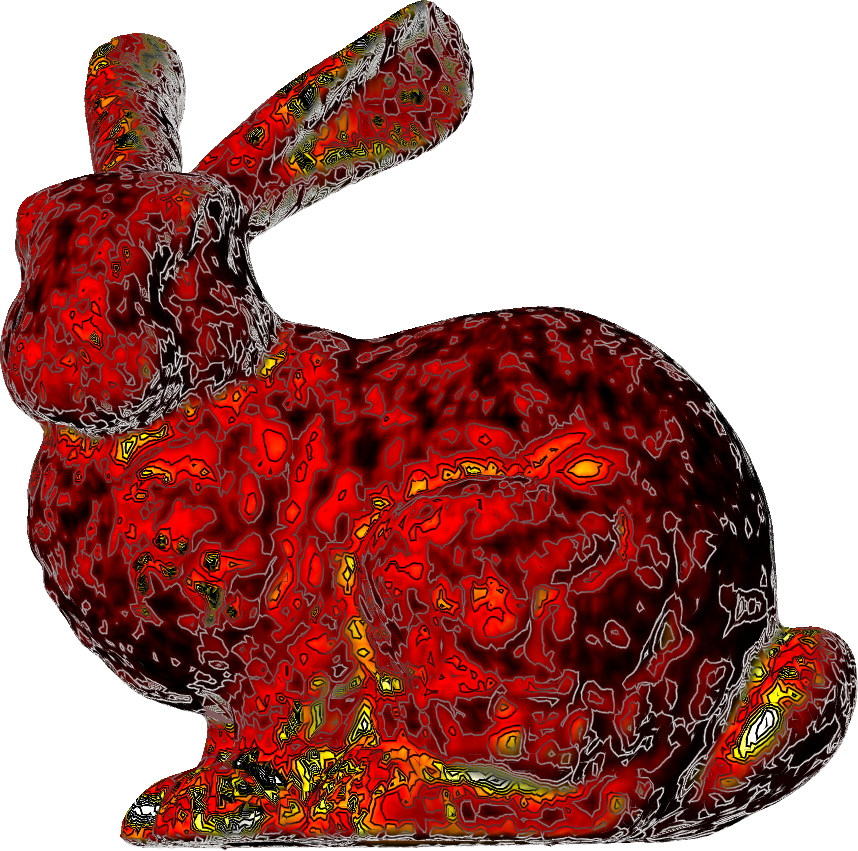
\includegraphics[width=1.0\linewidth,height=0.3\textheight,keepaspectratio]{data/acquired_meshes/bun_zipper_edited_r1_n4_v256_funcvals_isolines_10iter.png}
		\caption{Stanford Bunny 10iter isolines}\label{fig:bun.d}
	\end{subfigure}

	\bigskip
	\begin{subfigure}[b]{0.48\linewidth}
		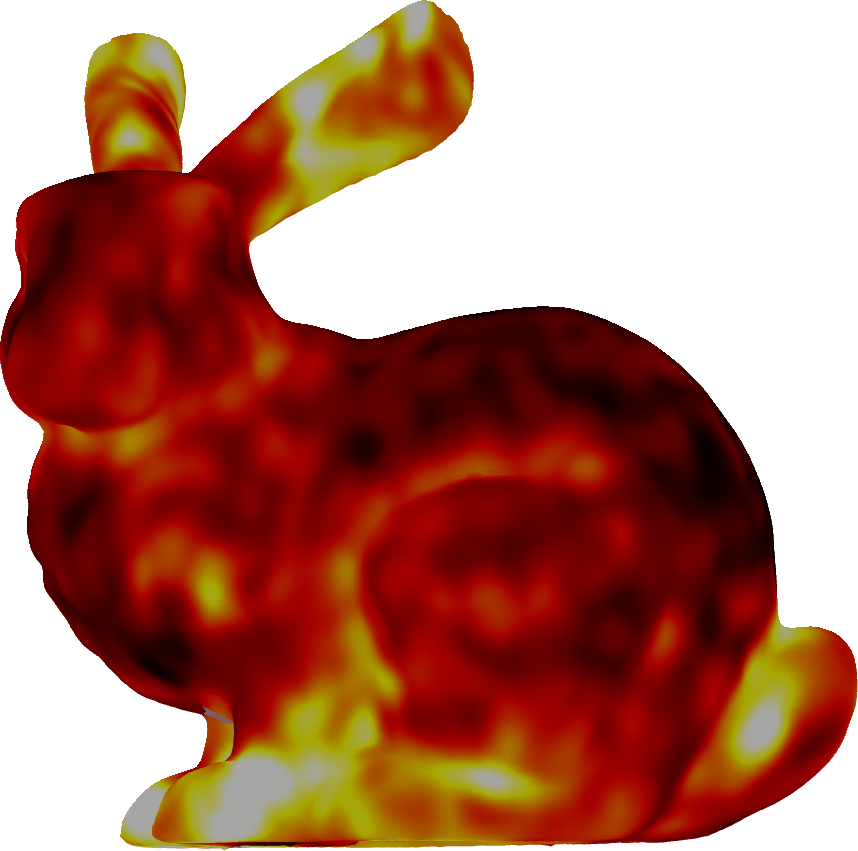
\includegraphics[width=1.0\linewidth,height=0.3\textheight,keepaspectratio]{data/acquired_meshes/bun_zipper_edited_r1_n4_v256_funcvals_100iter.png}
		\caption{Stanford Bunny Wireframe}\label{fig:bun.e}
	\end{subfigure}
	\begin{subfigure}[b]{0.48\linewidth}
		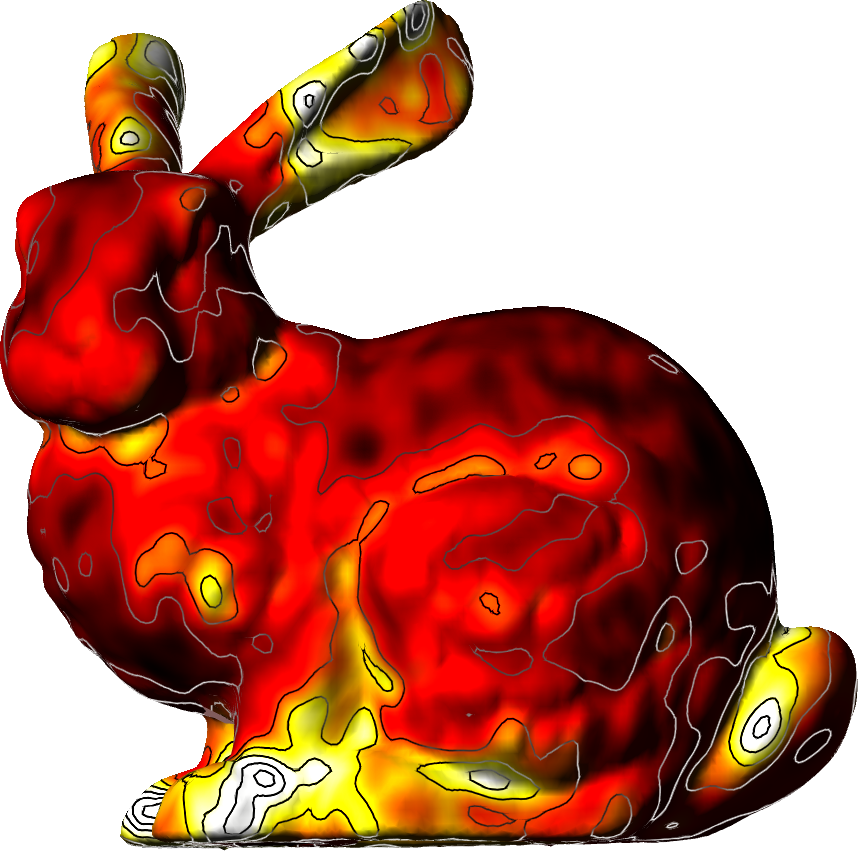
\includegraphics[width=1.0\linewidth,height=0.3\textheight,keepaspectratio]{data/acquired_meshes/bun_zipper_edited_r1_n4_v256_funcvals_isolines_100iter.png}
		\caption{Stanford Bunny 100iter isolines}\label{fig:bun.f}
	\end{subfigure}}
	{\caption[Stanford Bunny]{Stanford Bunny\ldots}\label{fig:bun}}
\end{figure}



\section{Evaluation}
\subsection{Compute Times}

Figure~\ref{fig:computeTimesLP} shows how compute times increase linearly with both mesh size and number of iterations in a very predictable way when total compute time is at least 0.1 seconds, and less predictable for shorter periods do to the nature of thread optimization at the processor level and variable memory read times.\todoResearch{add formula for timing (or at least ref to it) here.}\todoResearch{process time noise at very fast speeds}
\begin{figure}[ht]
	\centering
	\includegraphics[width=1.0\linewidth,height=1.0\textheight,keepaspectratio]{figures/computeTimesLinespoints.png}
	\RawCaption{\caption[Compute Times - Linespoints]{Compute Times of Applying
		the	One-Ring Filter for Selected Numbers of Iterations onto Acquired and
		Synthetic 3D Meshes of Varying Sizes}
		\label{fig:computeTimesLP}}
\end{figure}

Figure~\ref{fig:computeTimesS} shows how compute times increase with both meshsize and number of iterations.\todoCitation{https://en.wikipedia.org/wiki/Euler_characteristic#Polyhedra}
\begin{figure}[ht]
	\centering
	\includegraphics[width=1.0\linewidth,height=1.0\textheight,keepaspectratio]{figures/computeTimesScatter.png}
	\RawCaption{\caption[Compute Times - Scatter]{Compute Times for Different
		Hardware Configurations by increaseing Mesh Size and Filter Iterations}
		\label{fig:computeTimesS}}
\end{figure}

\begin{figure}[ht]
	\centering
	\includegraphics[width=1.0\linewidth,height=1.0\textheight,keepaspectratio]{figures/numFacesByVerticesGoTo2.png}
	\RawCaption{\caption[Ratio of Faces / Vertices]{Ratio of Faces to Vertices by
		Increasing Vertex Count}
		\label{fig:ratioFacesVertices}}
\end{figure}





\section{Summary}
Lorem ipsum dolor sit amet, consectetur adipiscing elit. Morbi tincidunt eget
ipsum eu iaculis. Cras vel sem eu velit eleifend porta vel sit amet massa. Etiam
a posuere nunc. Aenean aliquam viverra dapibus. Aliquam ac eros a purus feugiat
rhoncus. Donec faucibus ut nibh ut cursus. Aliquam erat volutpat. Proin efficitur
nulla sit amet iaculis condimentum. Cras placerat leo vitae venenatis feugiat. In
hac habitasse platea dictumst. Orci varius natoque penatibus et magnis dis
parturient montes, nascetur ridiculus mus. In aliquet sagittis dui eu pulvinar.
Morbi a arcu eu dolor sagittis varius. Aliquam dignissim tortor sed tortor
suscipit, eget imperdiet mauris convallis.
